% From Disruption to Agency — archival Beamer edition
% Companion to index.html (the reveal.js web deck). Content is kept in sync
% by hand; see README.md for the relationship between the two.
\documentclass[10pt,aspectratio=1610]{beamer}

\usepackage[utf8]{inputenc}
\usepackage[T1]{fontenc}
\usepackage{lmodern}
\usepackage{graphicx}
\usepackage{xcolor}
\usepackage{csquotes}
\usepackage{hyperref}

\usetheme{default}
\usecolortheme{default}
\setbeamertemplate{navigation symbols}{}

% ---- Palette: matches index.html's light-mode CSS variables, since a
% print-archival PDF should default to a light, ink-friendly background
% rather than the web deck's dark theme. ----
\definecolor{gktaccent}{HTML}{B8862F}  % amber  — headings / structure
\definecolor{gktaccent2}{HTML}{3F7A52} % sage   — emphasis / lead text
\definecolor{gktink}{HTML}{1C1C1C}
\definecolor{gktmuted}{HTML}{6B6B6B}
\definecolor{gktborder}{HTML}{E1DED7}

\setbeamercolor{normal text}{fg=gktink,bg=white}
\setbeamercolor{frametitle}{fg=gktaccent,bg=white}
\setbeamercolor{title}{fg=gktaccent}
\setbeamercolor{subtitle}{fg=gktaccent2}
\setbeamercolor{structure}{fg=gktaccent}
\setbeamercolor{itemize item}{fg=gktaccent}
\setbeamercolor{block title}{fg=gktaccent2}
\setbeamerfont{frametitle}{series=\bfseries}
\setbeamertemplate{itemize items}[circle]

\setbeamertemplate{footline}{%
  \hfill\footnotesize\color{gktmuted}%
  \insertframenumber{}/\inserttotalframenumber\hspace{1em}\vspace{4pt}%
}

\hypersetup{
  colorlinks=true,
  linkcolor=gktaccent2,
  urlcolor=gktaccent2,
  pdftitle={From Disruption to Agency: AI, Computing Cultures, and the Future of Digital Ethics},
  pdfauthor={George K. Thiruvathukal},
}

% ---- Small helpers mirroring the web deck's CSS classes ----
\newcommand{\lead}[1]{{\color{gktaccent2}#1}}
\newcommand{\accentterm}[1]{\textcolor{gktaccent2}{#1}}
\newcommand{\chaptertag}[1]{%
  \vfill{\footnotesize\color{gktmuted}\hrule height 0.4pt\vspace{4pt}CHOC --- #1\par}%
}
\newcommand{\noteinline}[1]{{\footnotesize\color{gktmuted}#1\par}}
\newcommand{\quoteblock}[2]{%
  \begin{quote}\color{gktink}\itshape\enquote{#1}\end{quote}
  {\footnotesize\color{gktmuted}--- #2\par}
}

\title{From Disruption to Agency}
\subtitle{AI, Computing Cultures, and the Future of Digital Ethics}
\author{George K. Thiruvathukal}
\date{}

\begin{document}

% ============================================================
% 1 · TITLE
% ============================================================
\begin{frame}[plain]
\centering
{\Large\bfseries\color{gktaccent}From Disruption to Agency}\\[0.6em]
{\large\color{gktaccent}AI, Computing Cultures, and the Future of Digital Ethics}\\[1em]
\lead{\small A talk drawn from \emph{History of Computing and Its Cultures: From Calculating to
Convergence} (in press for 2026--2027) by David B. Dennis and George K. Thiruvathukal (speaker)}\\[1.2em]
{\normalsize George K. Thiruvathukal, PhD}\\[0.4em]
{\footnotesize\color{gktmuted}
\href{https://www.luc.edu/cs/aboutus/people/profiles/thiruvathukalgeorgek.shtml}{Professor and Chairperson, Computer Science, Loyola University Chicago} ---
\href{mailto:gthiruvathukal@luc.edu}{gthiruvathukal@luc.edu} (preferred)\\
\href{https://www.alcf.anl.gov/about/people/george-k-thiruvathukal}{Visiting Computer Scientist, Argonne National Laboratory} ---
\href{mailto:gkt@anl.gov}{gkt@anl.gov}\\[0.3em]
\href{https://keylinks.gkt.sh}{keylinks.gkt.sh} (web)\\[0.6em]
\href{https://www.luc.edu/digitalethics/events/annualsymposium/}{15th Annual International Symposium on Digital Ethics: MAGIS --- September 28--29, 2026}\\[0.6em]
DOI: \href{https://doi.org/10.6084/m9.figshare.33944386}{10.6084/m9.figshare.33944386}
}
\end{frame}

% ============================================================
% 1B · QR CODES (post-title)
% ============================================================
\begin{frame}[plain]
\centering
{\Large\bfseries\color{gktaccent}Follow Along}\\[1em]
\begin{columns}[T]
\column{0.5\textwidth}
\centering

\includegraphics[height=3.6cm]{images/qr-talk.png}\\[0.4em]
\footnotesize This talk\\\href{https://talks.gkt.sh/luc-digital-ethics-2026/}{talks.gkt.sh/luc-digital-ethics-2026}
\column{0.5\textwidth}
\centering

\includegraphics[height=3.6cm]{images/qr-keylinks.png}\\[0.4em]
\footnotesize Find me\\\href{https://keylinks.gkt.sh}{keylinks.gkt.sh}
\end{columns}
\end{frame}

% ============================================================
% 2 · THESIS
% ============================================================
\begin{frame}{The Core Thesis}
\begin{itemize}
\item The opening claim: \enquote{Computing came from culture, and then culture increasingly was shaped by computing.}
\item A reversal: computation began as a \accentterm{cultural artifact} --- tallies, abaci --- before it became a \accentterm{world-making environment}.
\item Digital ethics is not a patch for biased models. It is a question about what computation has always done to culture.
\end{itemize}
\noteinline{If that reversal is right, no computing technology's ethical questions arrive from nowhere. They are old questions wearing a new interface --- and this talk is a history of the interfaces, not a talk about any one of them.}
\chaptertag{\enquote{The Core Thesis}}
\end{frame}

% ============================================================
% 3 · THEN/NOW BOOKEND
% ============================================================
\begin{frame}{Two Thresholds, Both Missed at the Time}
\begin{columns}[T]
\column{0.5\textwidth}
\centering
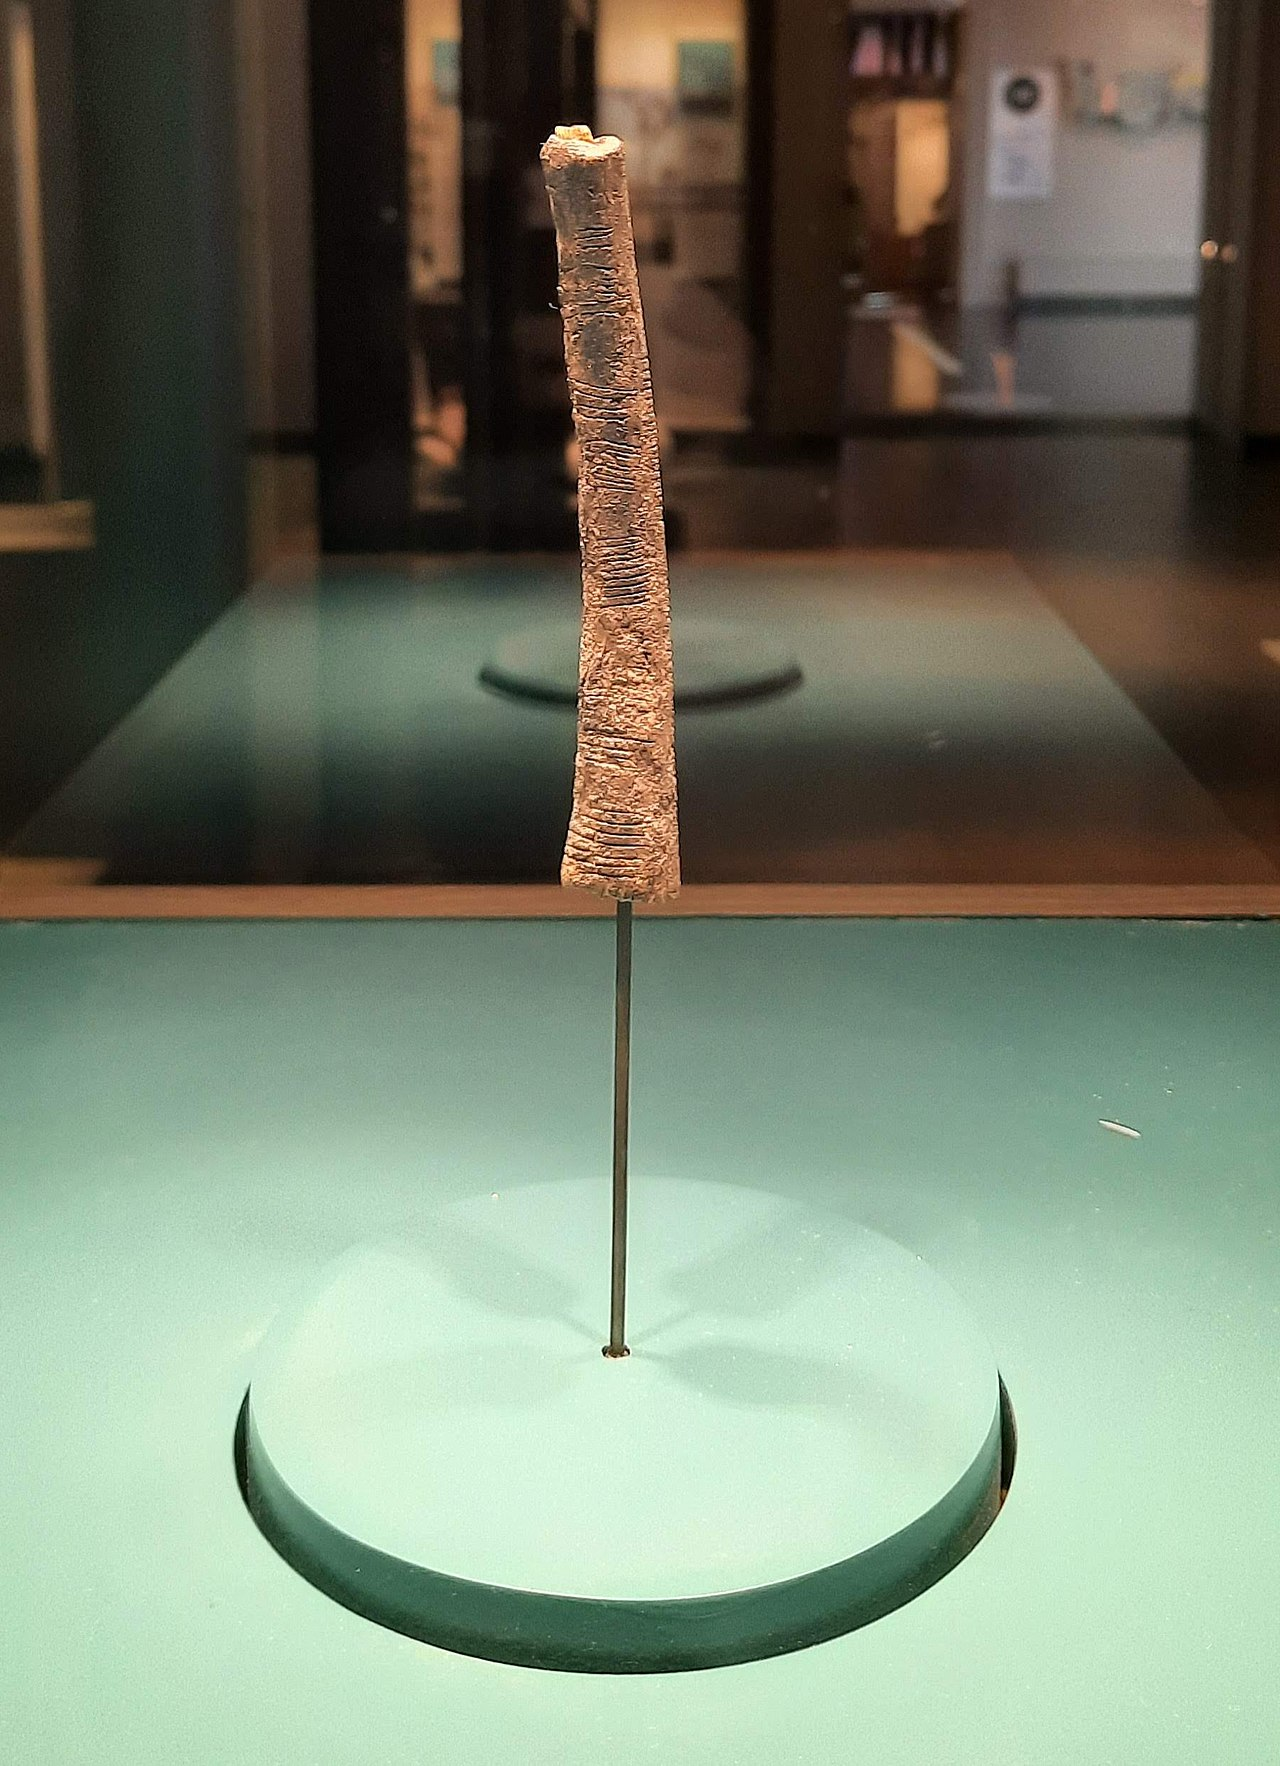
\includegraphics[height=3.4cm,keepaspectratio]{images/ishango-bone.jpg}\\
{\tiny\color{gktmuted}Ishango Bone. JhowieNitnek, Wikimedia Commons, CC BY-SA 4.0.}\\[0.4em]
\raggedright\footnotesize c. 20{,}000 BCE --- notches that made \enquote{one} \accentterm{separable from any particular object}: the first abstraction underlying computation.
\column{0.5\textwidth}
\centering
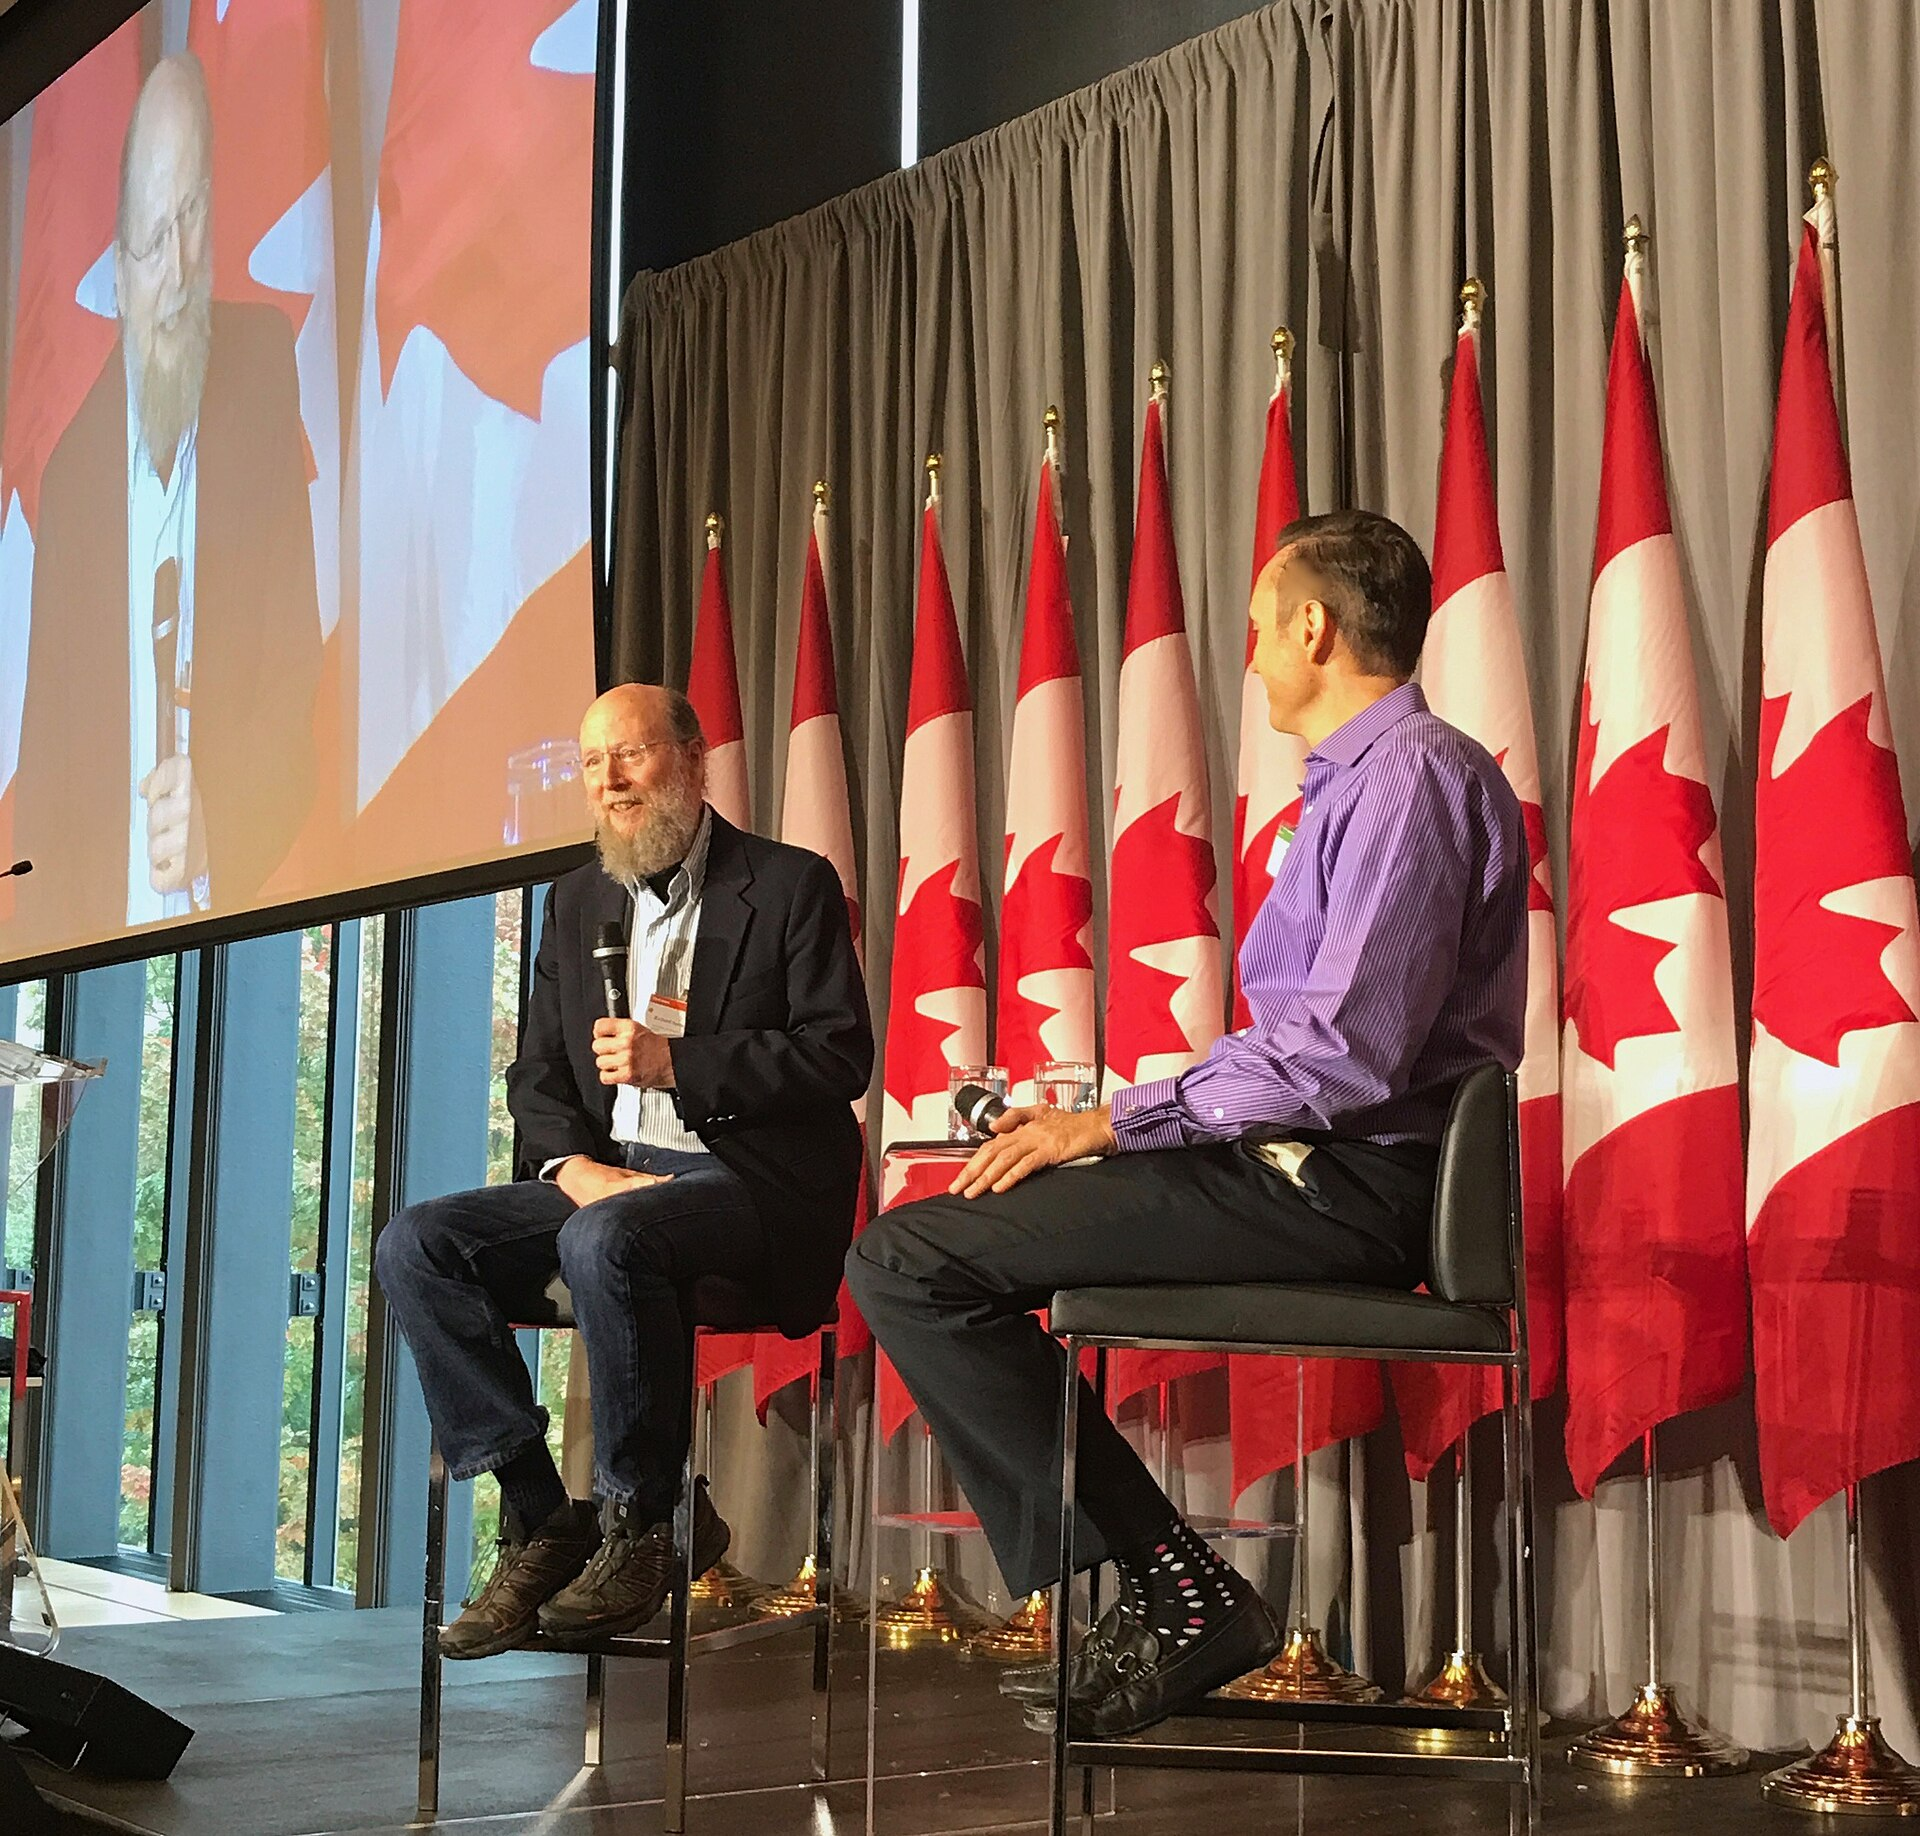
\includegraphics[height=3.4cm,keepaspectratio]{images/alpha-go.jpg}\\
{\tiny\color{gktmuted}AlphaGo / reinforcement learning. Wikimedia Commons, public domain.}\\[0.4em]
\raggedright\footnotesize 2010s --- deep learning, transformers, BERT, GPT-2: \enquote{submerged infrastructure} that \enquote{few\ldots{} imagined\ldots{} could become the basis for general-purpose conversational agents.}
\end{columns}
\noteinline{Same pattern, both times: the abstraction advances quietly, and only in hindsight does it look like a threshold. That is the case against Kurzweil's speculative singularity --- and for the one CHOC says we already lived, in 2020.}
\chaptertag{\enquote{Paleolithic Numbers and Calculating} $\cdot$ \enquote{Data, AI, and the Edge of Automation}}
\end{frame}

% ============================================================
% 4 · FAUSTIAN-TURING PLANT
% ============================================================
\begin{frame}{A Hybrid Figure, Centuries in the Making}
\begin{columns}[T]
\column{0.55\textwidth}
\begin{itemize}
\item The \textbf{Faustian Type}: since Babbage's engines, \enquote{restless for novelty and progress} --- the drive to build and extend human reach.
\item The \textbf{Turing Type}: since Hollerith's punched cards and Turing's abstract computer, learned to \enquote{think with, design, and command} those machines.
\item CHOC: the two coexisted through most of the twentieth century --- \enquote{explorers and experts\ldots{} publics and professionals} --- and merged into \enquote{everyday fact} only in the 2010s.
\end{itemize}
\column{0.45\textwidth}
\quoteblock{We are both monstrous and marvelous, born of ambition and algorithm, living within a culture that is no longer separable from its machines.}{\emph{History of Computing and Its Cultures}}
\end{columns}
\chaptertag{\enquote{Conclusion: The Cultural-Computing Singularity}}
\end{frame}

% ============================================================
% 5 · PART 2 DIVIDER
% ============================================================
\section{Six Lenses, One Continuous Argument}
\begin{frame}[plain]
\centering
{\Large\bfseries\color{gktaccent}Six Lenses, One Continuous Argument}\\[1em]
\lead{\normalsize Automation $\cdot$ Agency $\cdot$ Accountability $\cdot$ Access $\cdot$ Labor $\cdot$ Environmental Cost}
\end{frame}

% ============================================================
% 6 · CH2 LEIBNIZ
% ============================================================
\begin{frame}{Automating the Drudgery}
\begin{columns}[T]
\column{0.55\textwidth}
\begin{itemize}
\item Leibniz on hand calculation: \enquote{unworthy of excellent men to lose hours like slaves.}
\item The oldest automation pitch on record: free minds for \emph{higher} work.
\item Three and a half centuries later, the pitch is unchanged --- only the machine is.
\end{itemize}
\chaptertag{\enquote{Paleolithic to Scientific Revolution}}
\column{0.45\textwidth}
\centering
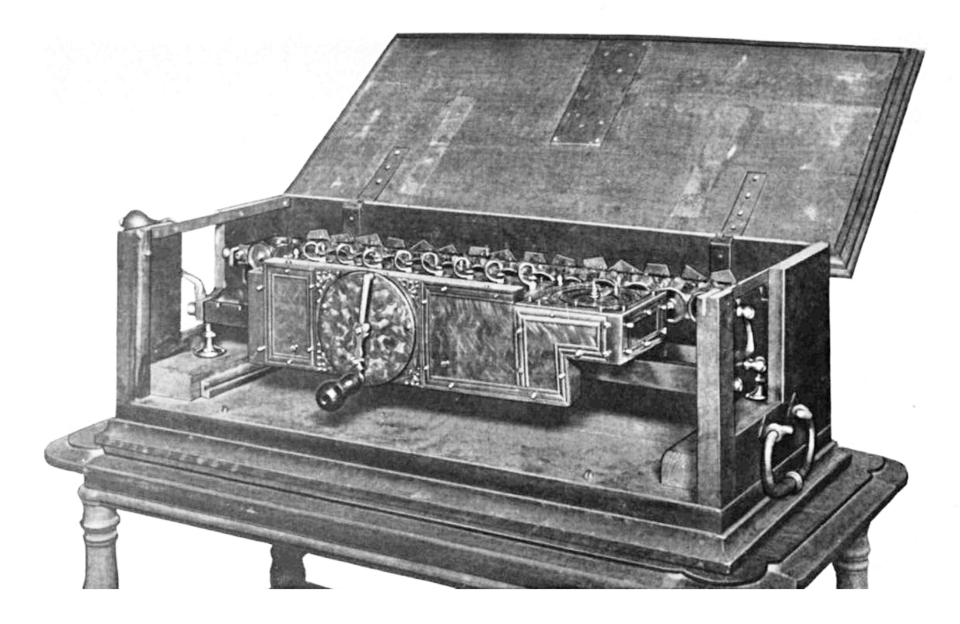
\includegraphics[height=4cm,keepaspectratio]{images/leibniz-drum-calculator.png}\\
{\tiny\color{gktmuted}Leibniz Stepped Reckoner. J.\,A.\,V. Turck, Wikimedia Commons, CC0.}
\end{columns}
\end{frame}

% ============================================================
% 7 · CH2 ACCESS
% ============================================================
\begin{frame}{Who Was Allowed to Count}
\begin{columns}[T]
\column{0.55\textwidth}
\begin{itemize}
\item Literacy and calculation were restricted to scribal elites for millennia.
\item Aristotle: mathematics arose where \enquote{the priestly class was allowed leisure.}
\item Access to computation has always tracked access to privilege.
\end{itemize}
\chaptertag{\enquote{Paleolithic to Scientific Revolution}}
\column{0.45\textwidth}
\centering
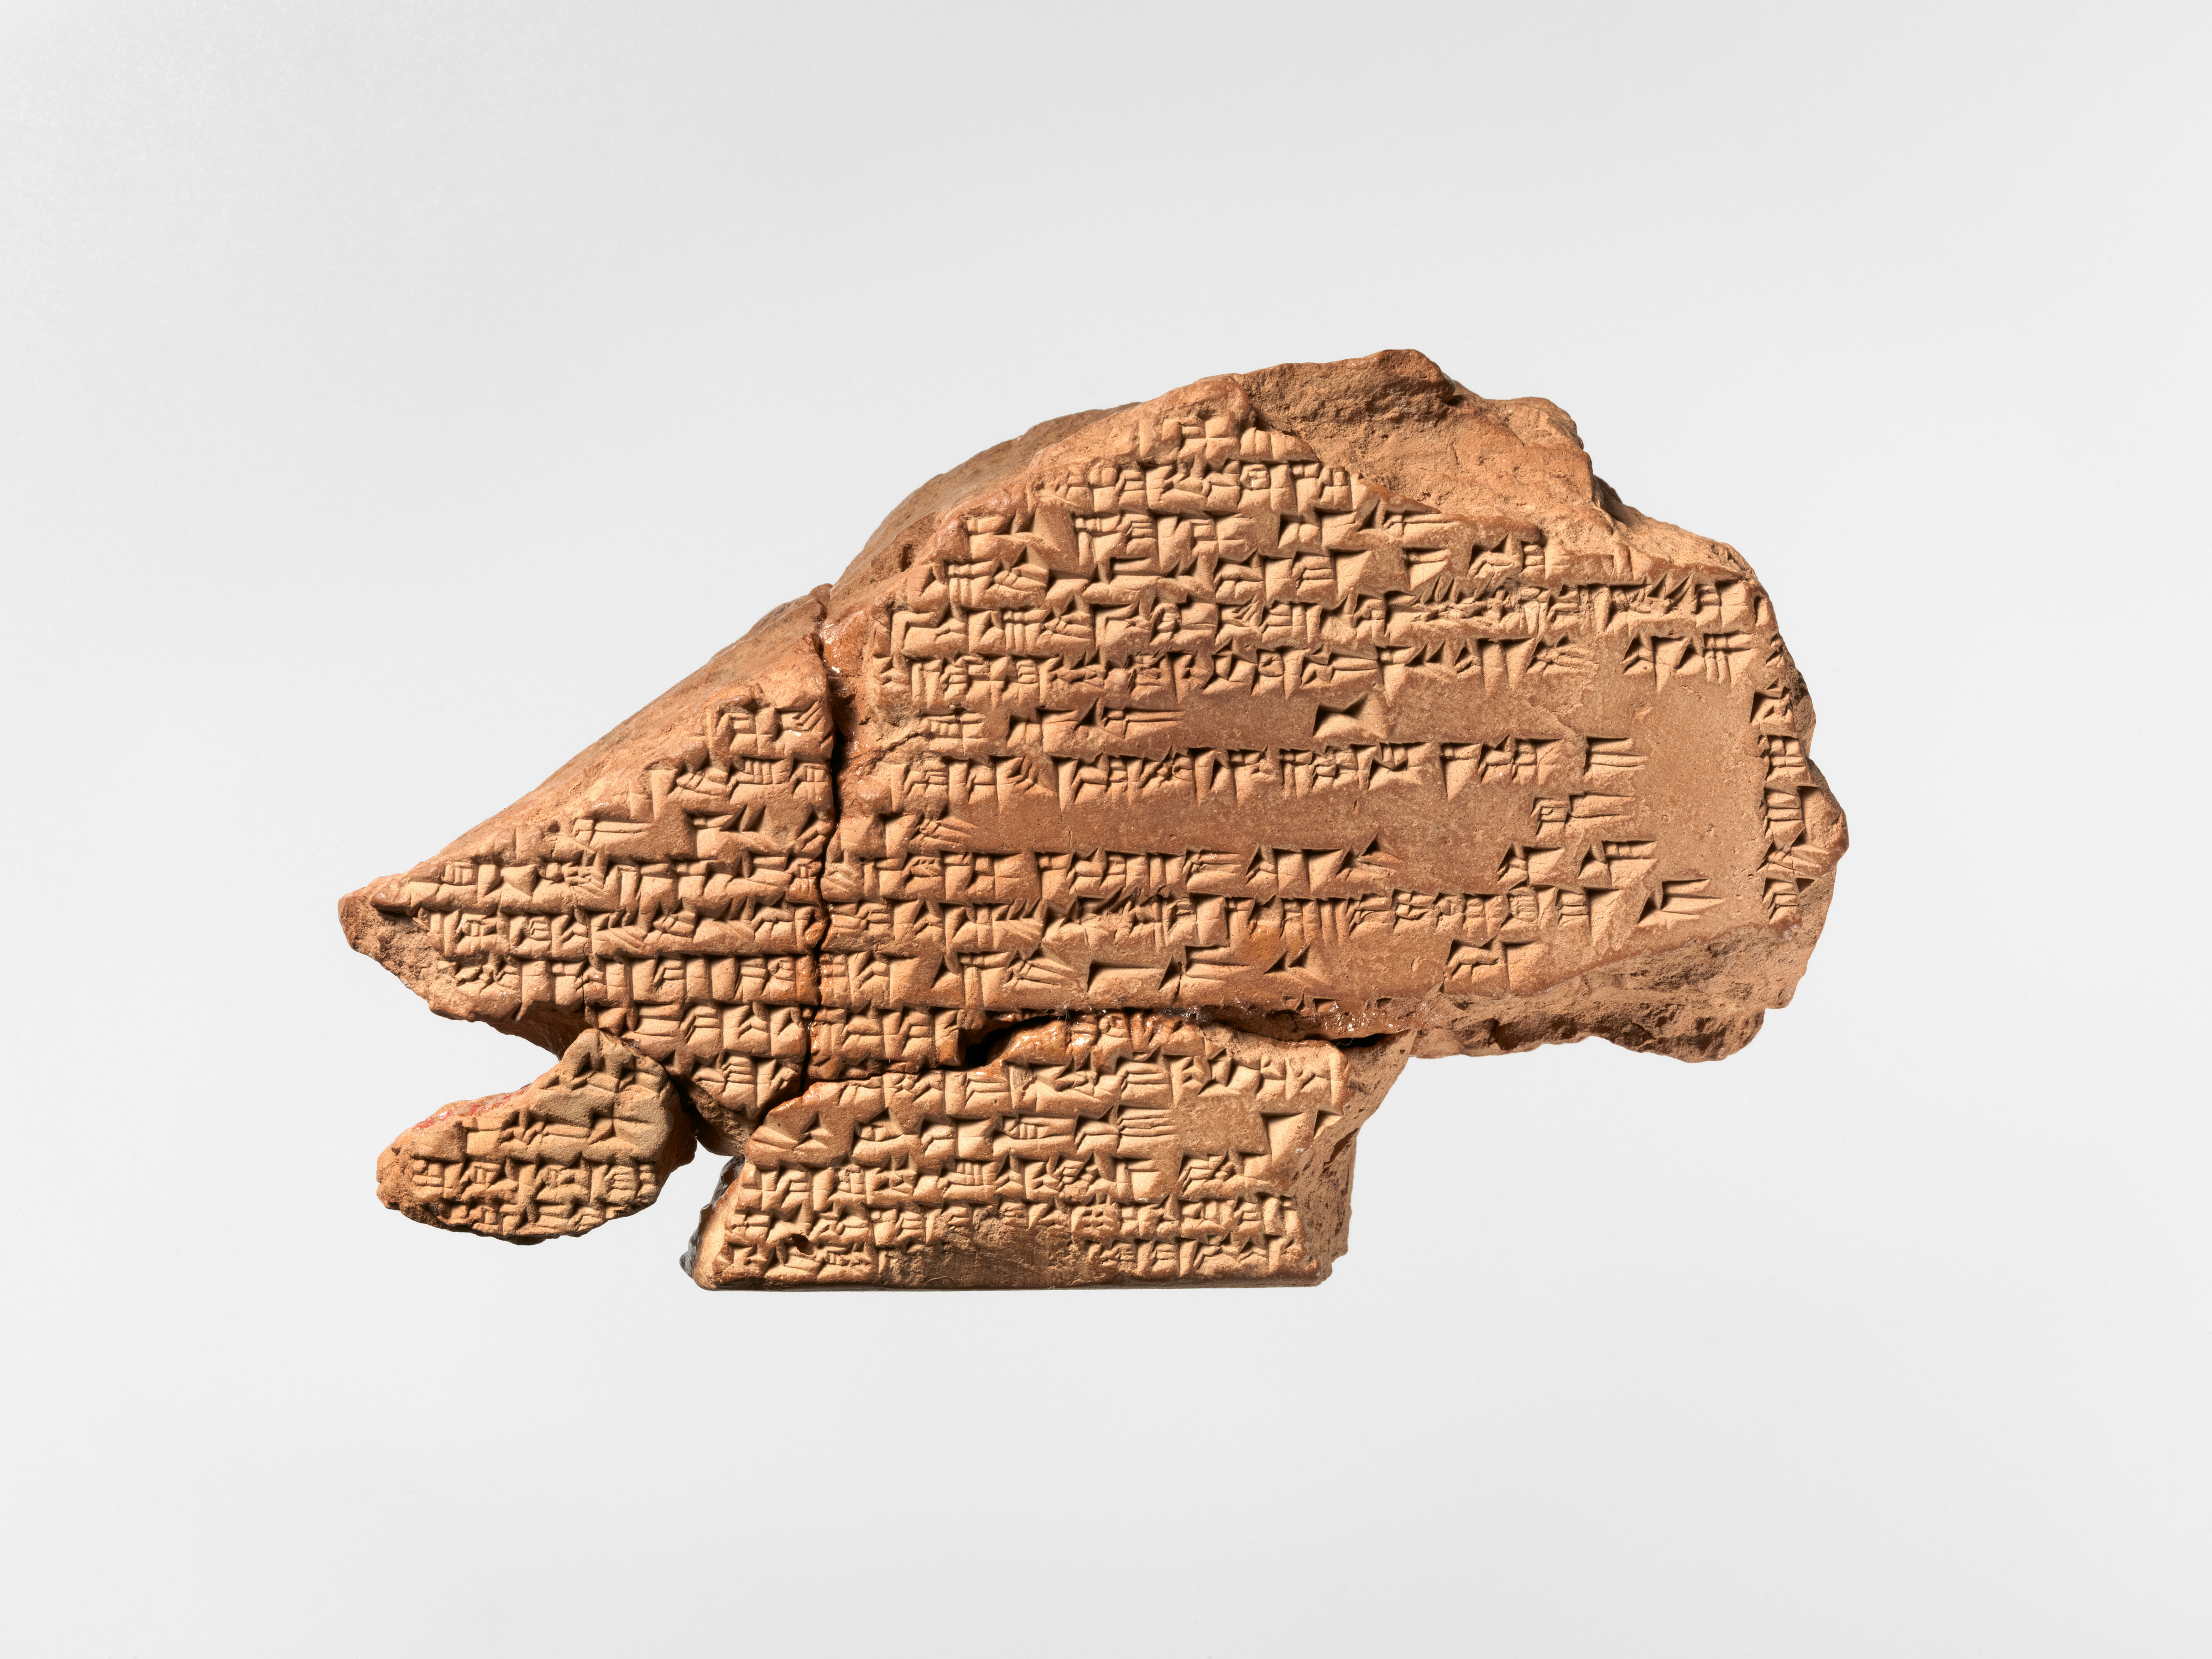
\includegraphics[height=4cm,keepaspectratio]{images/clay-tablet-cuneiform-2.jpg}\\
{\tiny\color{gktmuted}Cuneiform tablet, commentary on Enuma Anu Enlil. Wikimedia Commons, CC0.}
\end{columns}
\end{frame}

% ============================================================
% 8 · CH3 BABBAGE
% ============================================================
\begin{frame}{The Tables Crisis}
\begin{columns}[T]
\column{0.55\textwidth}
\begin{itemize}
\item Human \enquote{computers} produced error-prone astronomical/navigational tables.
\item Herschel: \enquote{an undetected error\ldots{} is like a sunken rock at sea.}
\item Babbage's Difference Engine mechanizes an \emph{existing} labor pipeline (de Prony's \textasciitilde{}100 human computers) --- automation formalizes, it doesn't invent.
\end{itemize}
\chaptertag{\enquote{Babbage, Lovelace, and the Analytical Engine}}
\column{0.45\textwidth}
\centering
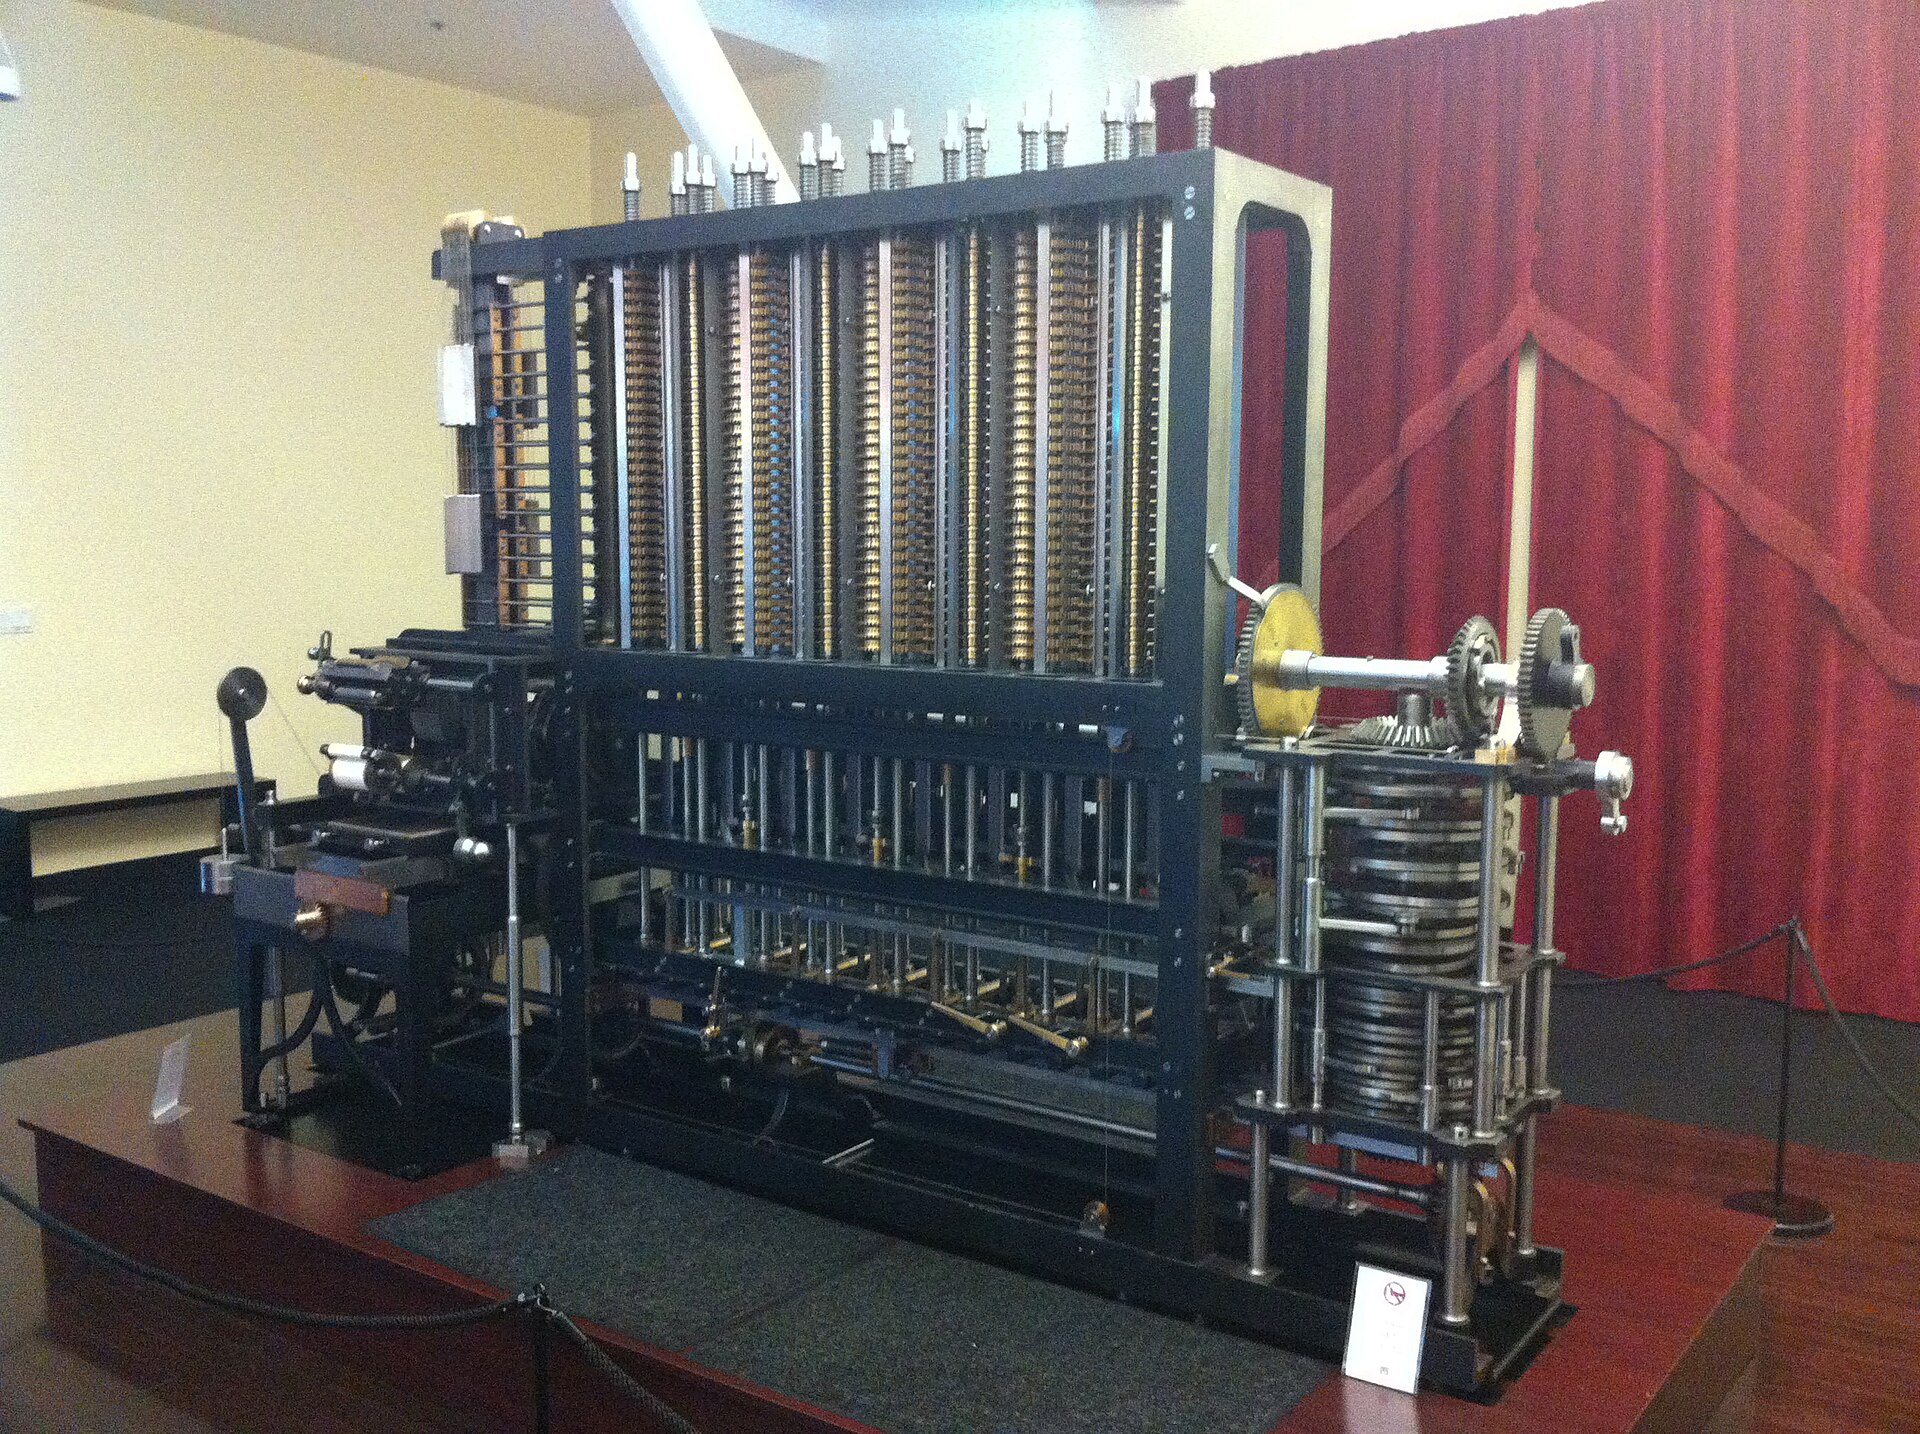
\includegraphics[height=4cm,keepaspectratio]{images/difference-engine.jpg}\\
{\tiny\color{gktmuted}Charles Babbage's Difference Engine No.\,2. Wikimedia Commons, public domain.}
\end{columns}
\end{frame}

% ============================================================
% 9 · CH3 LOVELACE
% ============================================================
\begin{frame}{The Counterpoint: Augmentation, Not Replacement}
\begin{columns}[T]
\column{0.55\textwidth}
\footnotesize CHOC's account of Lovelace's own speculation:
\quoteblock{She speculated that, given the right instructions, the Analytical Engine might compose music or create art.}{\emph{History of Computing and Its Cultures}, on Ada Lovelace}
\begin{itemize}
\item CHOC calls this \enquote{a vision of computing that anticipates the idea of computers as creative instruments, not just mathematical engines.}
\item Written before the Engine was ever built --- the earliest case for augmentation over replacement.
\end{itemize}
\chaptertag{\enquote{Babbage, Lovelace, and the Analytical Engine}}
\column{0.45\textwidth}
\centering
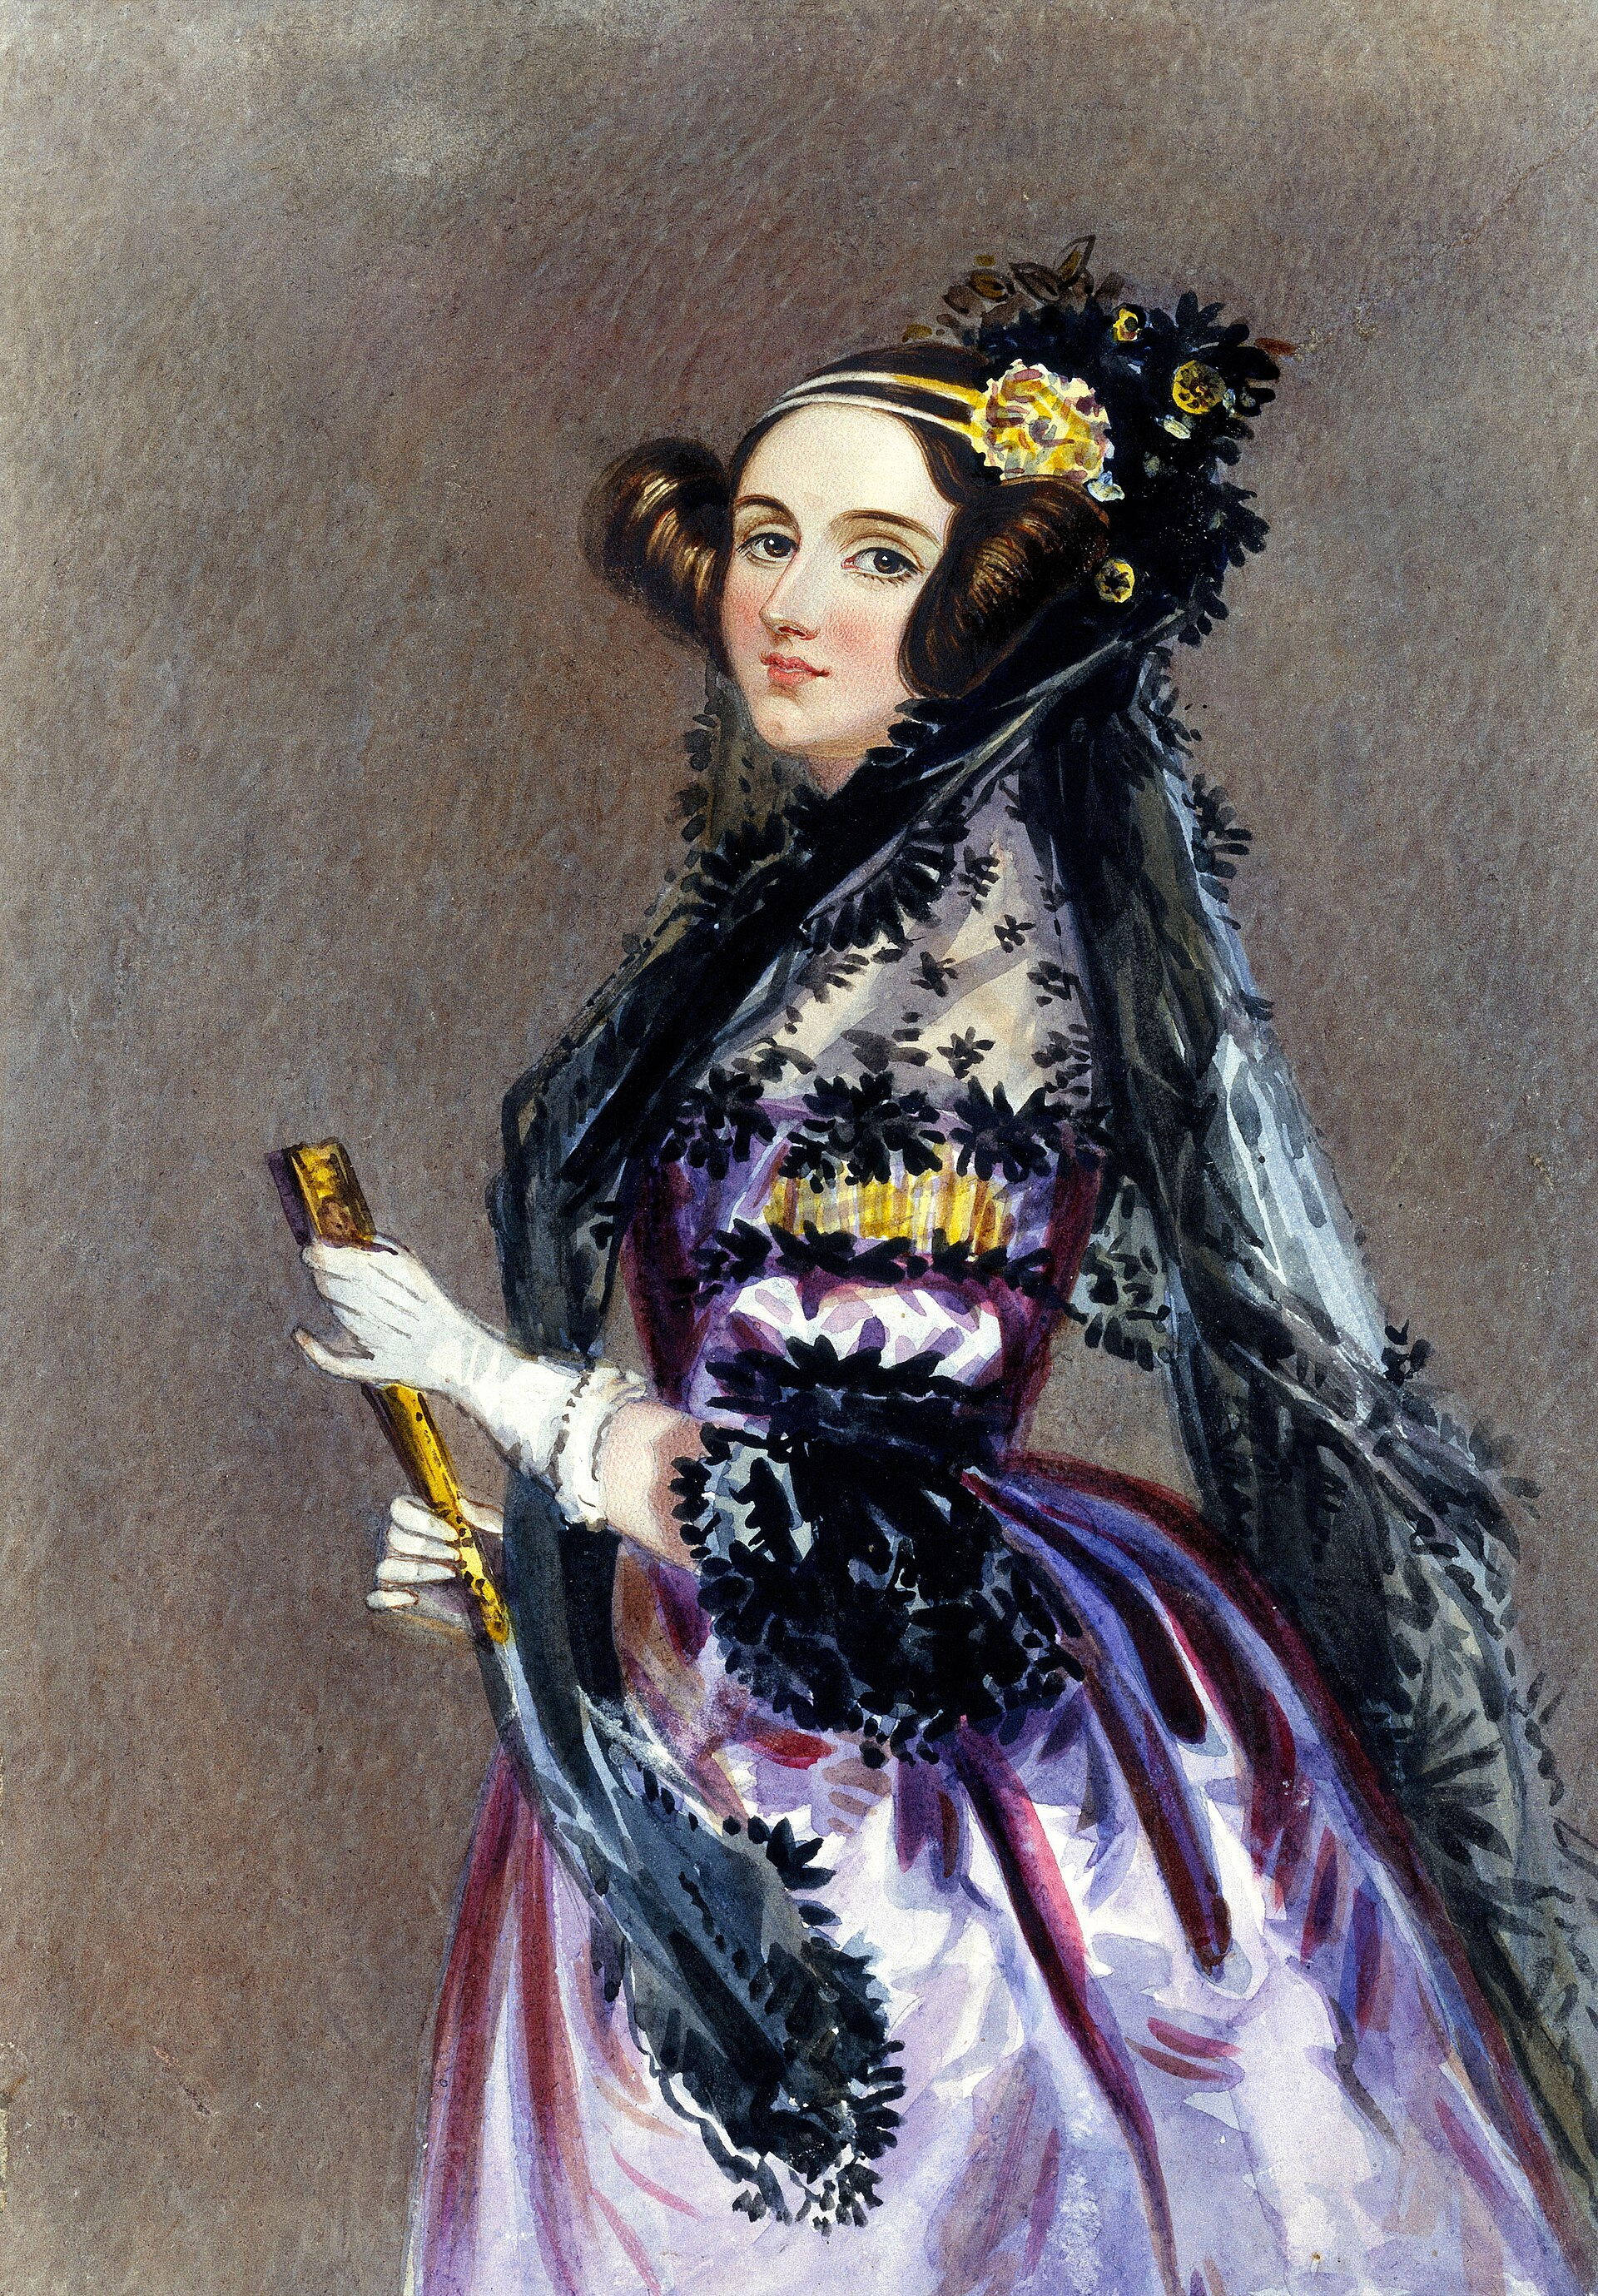
\includegraphics[height=4cm,keepaspectratio]{images/ada-lovelace-ppt0-history-slide13.jpg}\\
{\tiny\color{gktmuted}Portrait of Ada Lovelace, attr. Alfred Edward Chalon, ca. 1840. Wikimedia Commons, public domain.}
\end{columns}
\end{frame}

% ============================================================
% 10 · CH4 HOLLERITH
% ============================================================
\begin{frame}{Automation Answers an Overload Crisis}
\begin{columns}[T]
\column{0.55\textwidth}
\begin{itemize}
\item The 1880 U.S. census took nearly a decade to tabulate by hand.
\item Hollerith's punched cards: \emph{data}, not instructions --- a distinction computing would keep rediscovering for the next 140 years.
\item \enquote{Clerks became operators} --- the office workforce reorganized, not eliminated.
\end{itemize}
\chaptertag{\enquote{Hollerith, Punched Cards, and Business Machines}}
\column{0.45\textwidth}
\centering
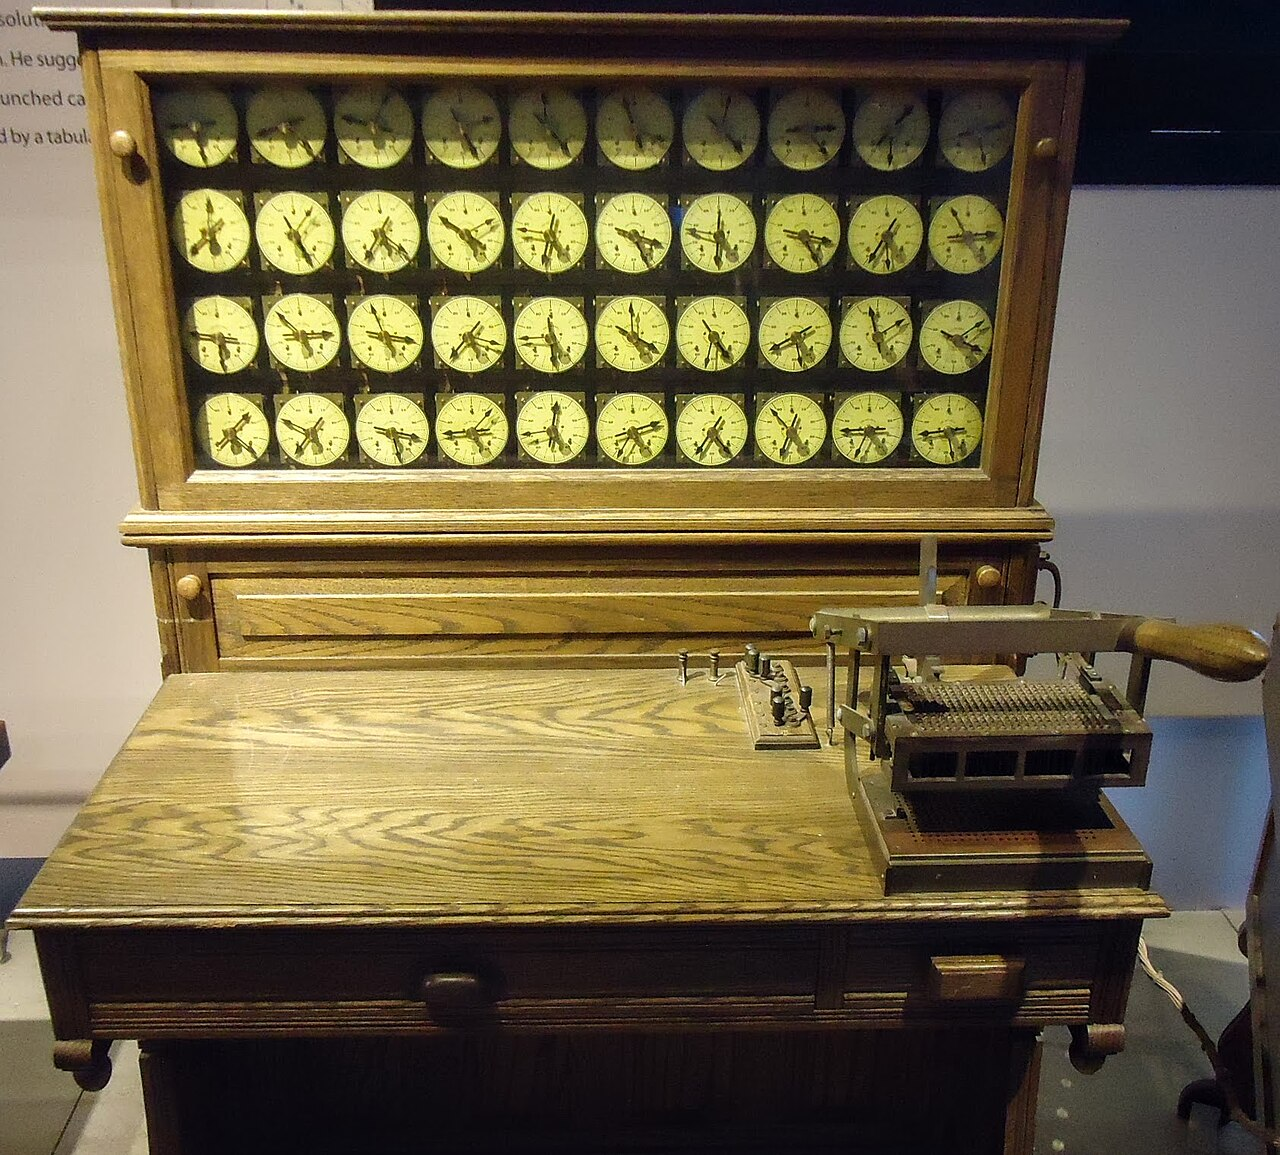
\includegraphics[height=4cm,keepaspectratio]{images/hollerith-tabulating.jpg}\\
{\tiny\color{gktmuted}Hollerith tabulating machine, Computer History Museum. Wikimedia Commons, public domain.}
\end{columns}
\end{frame}

% ============================================================
% 11 · CH4 ENVIRONMENTAL
% ============================================================
\begin{frame}{The Infrastructure Underneath}
\begin{itemize}
\item Millions of kilograms of gutta-percha harvested from Southeast Asia to insulate transatlantic cables.
\item CHOC's own words: \enquote{an early example of how global demand for `network infrastructure' could create unsustainable environmental and economic practices.}
\item Every convergence has had a material cost, paid somewhere else.
\end{itemize}
\chaptertag{\enquote{Hollerith, Punched Cards, and Business Machines}}
\end{frame}

% ============================================================
% 12 · CH5 LABOR
% ============================================================
\begin{frame}{The Computers Were Women}
\begin{columns}[T]
\column{0.55\textwidth}
\begin{itemize}
\item Human \enquote{computers} at Aberdeen, Bletchley Park, the Moore School --- mostly women, college-educated.
\item ENIAC's first programmers: Jean Jennings, Betty Snyder, Marlyn Wescoff, and others.
\item Their labor made the machine practical and flexible; credit did not follow.
\end{itemize}
\chaptertag{\enquote{WWII: From Ballistics to Electronic Computing}}
\column{0.45\textwidth}
\centering
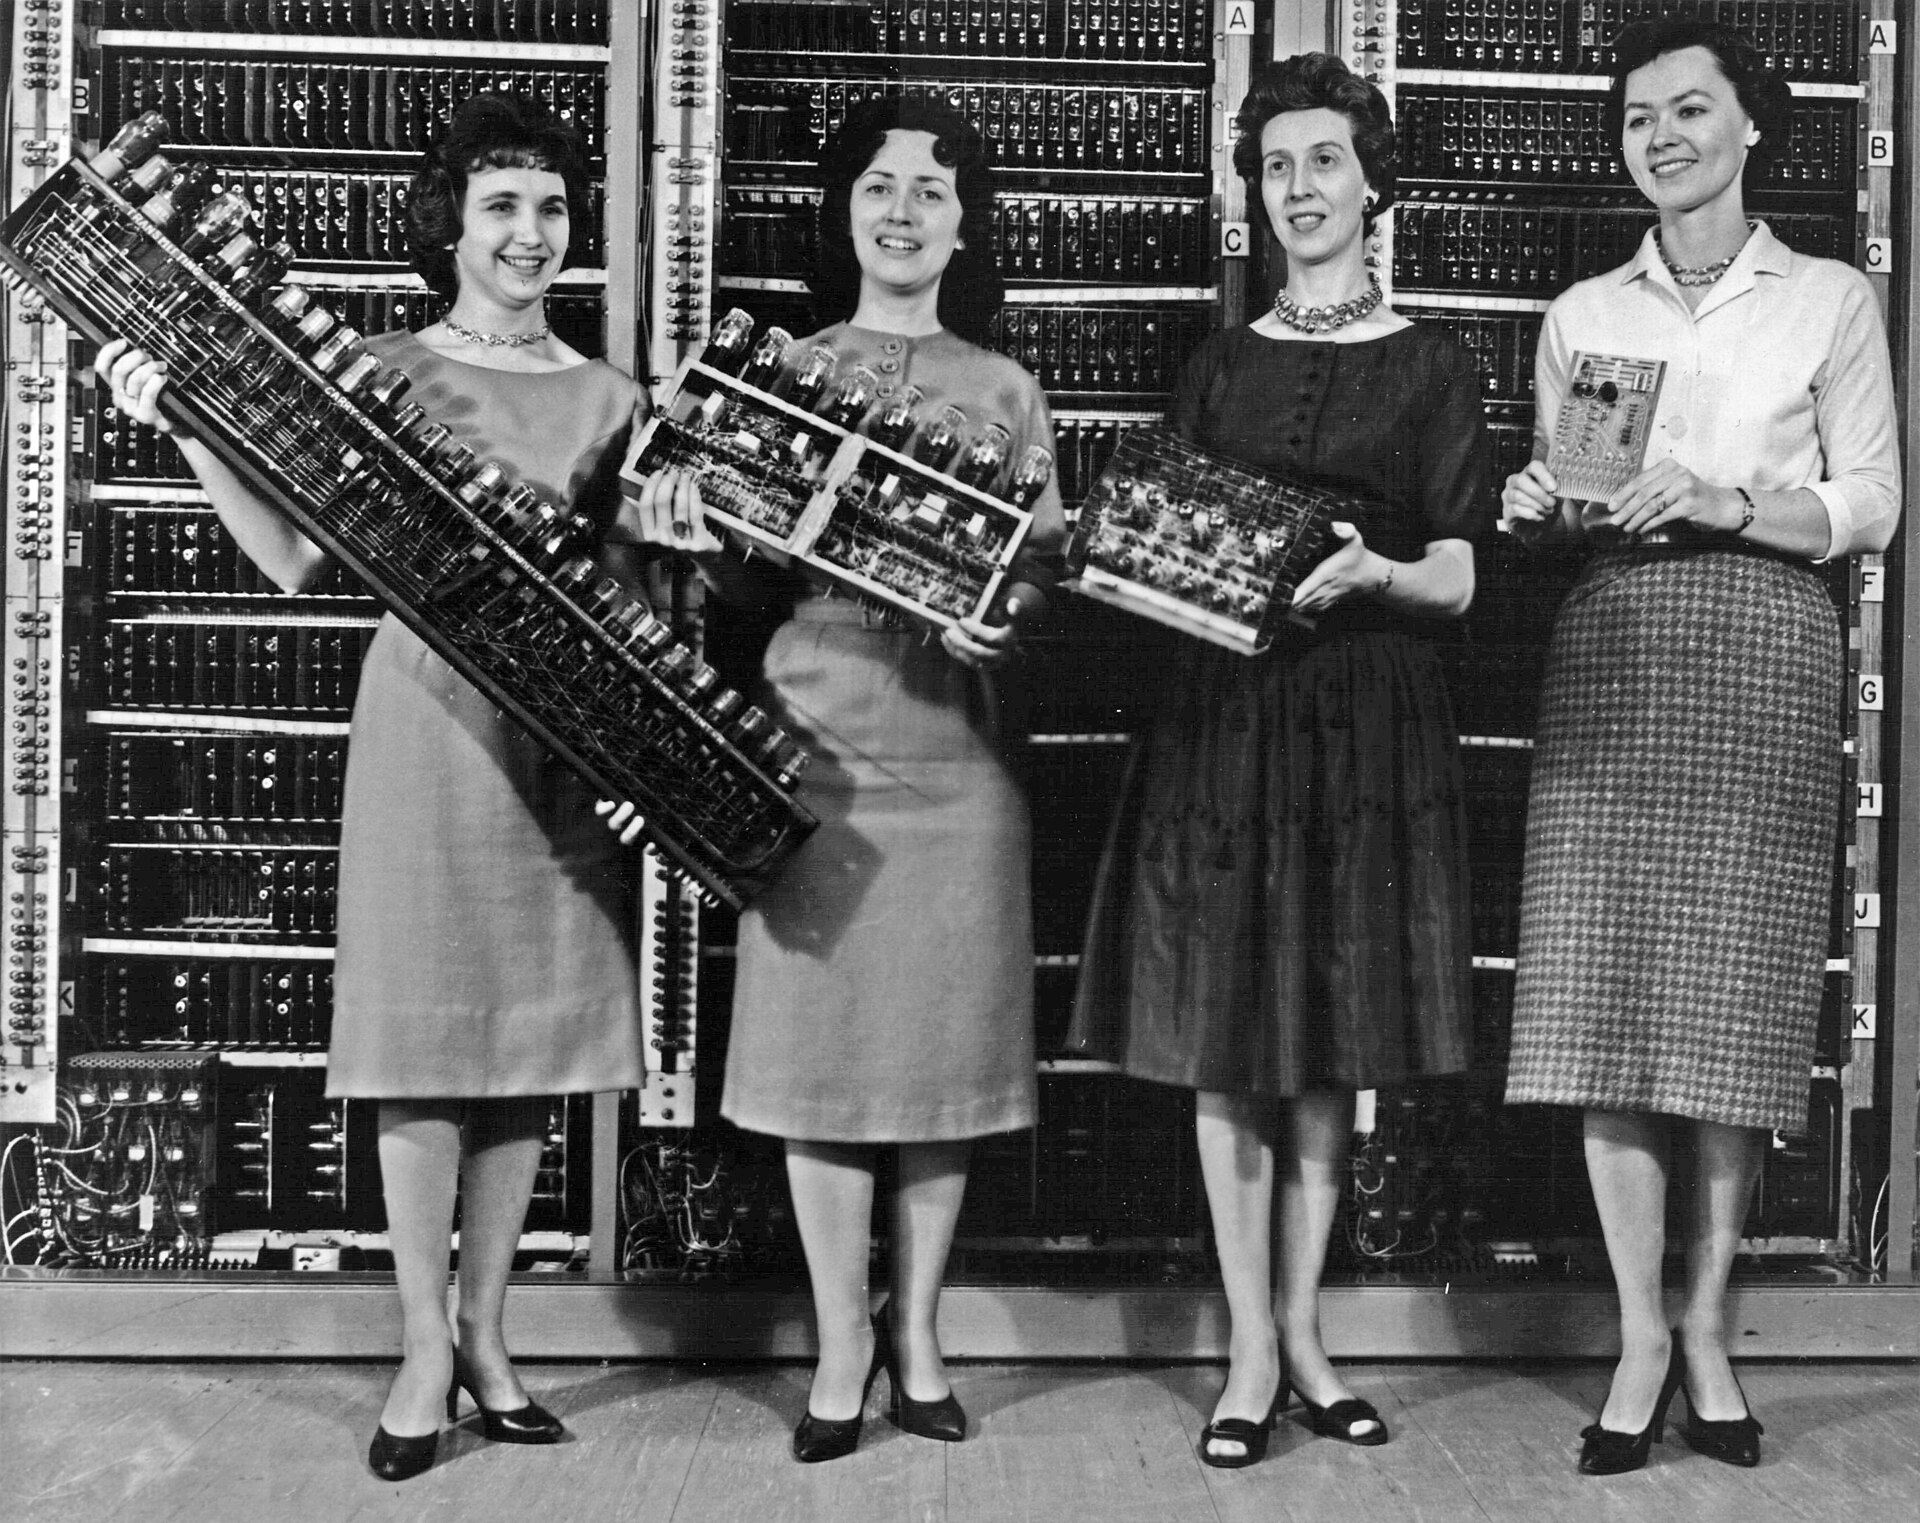
\includegraphics[height=4cm,keepaspectratio]{images/eniac-women-wiring-1.jpg}\\
{\tiny\color{gktmuted}Women holding parts of the first four Army computers. Wikimedia Commons, public domain.}
\end{columns}
\end{frame}

% ============================================================
% 12a · CH5 TURING MACHINE
% ============================================================
\begin{frame}{Computation Gets a Definition}
\begin{columns}[T]
\column{0.55\textwidth}
\begin{itemize}
\item 1936: Turing's paper on \enquote{computable numbers} introduces an abstract \enquote{universal machine.}
\item CHOC: it \enquote{offered the first rigorous definition of computation itself} --- a vocabulary for calculation as a general process, not a collection of ad hoc methods.
\item Decades of augmentation --- PCs, networks, the Web --- all stand on this one idea, long before any of them were called AI.
\end{itemize}
\chaptertag{\enquote{WWII: From Ballistics to Electronic Computing}}
\column{0.45\textwidth}
\centering
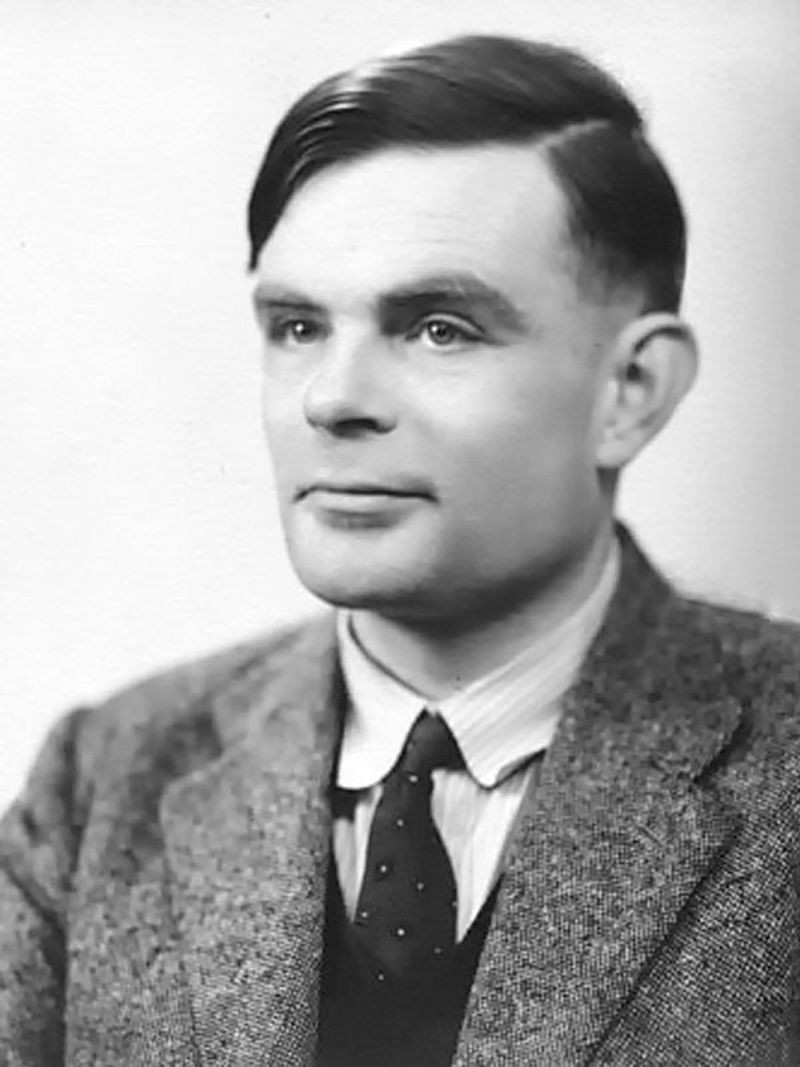
\includegraphics[height=4cm,keepaspectratio]{images/turing-image-01.jpg}\\
{\tiny\color{gktmuted}Alan Turing (1951). Wikimedia Commons, public domain.}
\end{columns}
\end{frame}

% ============================================================
% 13 · CH6 ACCOUNTABILITY
% ============================================================
\begin{frame}{Who Answers for the Machine's Judgment?}
\begin{columns}[T]
\column{0.55\textwidth}
\begin{itemize}
\item UNIVAC correctly forecasts the 1952 election from early returns.
\item Broadcasters initially distrust the prediction and downplay it on air.
\item The first public spectacle of, and public suspicion toward, machine judgment.
\end{itemize}
\chaptertag{\enquote{Mainframes and Cold War Systems}}
\column{0.45\textwidth}
\centering
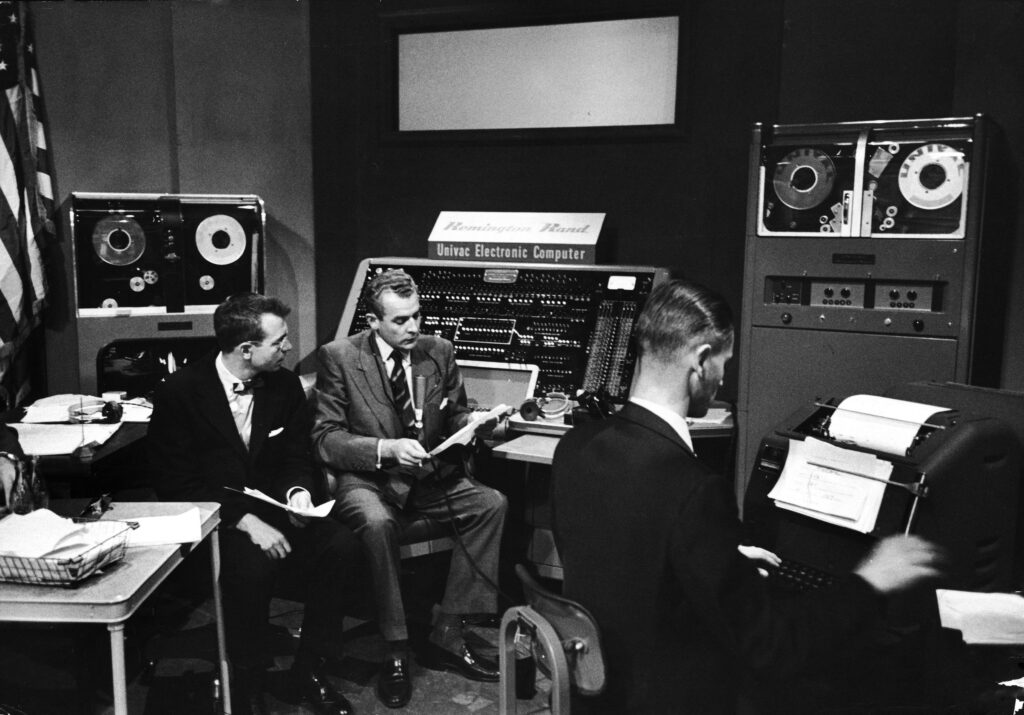
\includegraphics[height=4cm,keepaspectratio]{images/Univac-1952-LIFE-Picture-Collection-Al-Fenn.jpg}\\
{\tiny\color{gktmuted}Charles Collingwood with UNIVAC, 1952 election broadcast. Al Fenn/LIFE Picture Collection/Shutterstock.}
\end{columns}
\end{frame}

% ============================================================
% 14 · CH6 LABOR
% ============================================================
\begin{frame}{Same Technology, Reassigned Prestige}
\begin{columns}[T]
\column{0.55\textwidth}
\begin{itemize}
\item CHOC: early programming was \enquote{regarded as clerical work, suitable for women who had previously served as human `computers.'}
\item As complexity grew, it came to be \enquote{recognized as a skilled profession.}
\item The underlying labor --- transcription, checking, documentation --- didn't change. Its status did.
\end{itemize}
\chaptertag{\enquote{Mainframes and Cold War Systems}}
\column{0.45\textwidth}
\centering
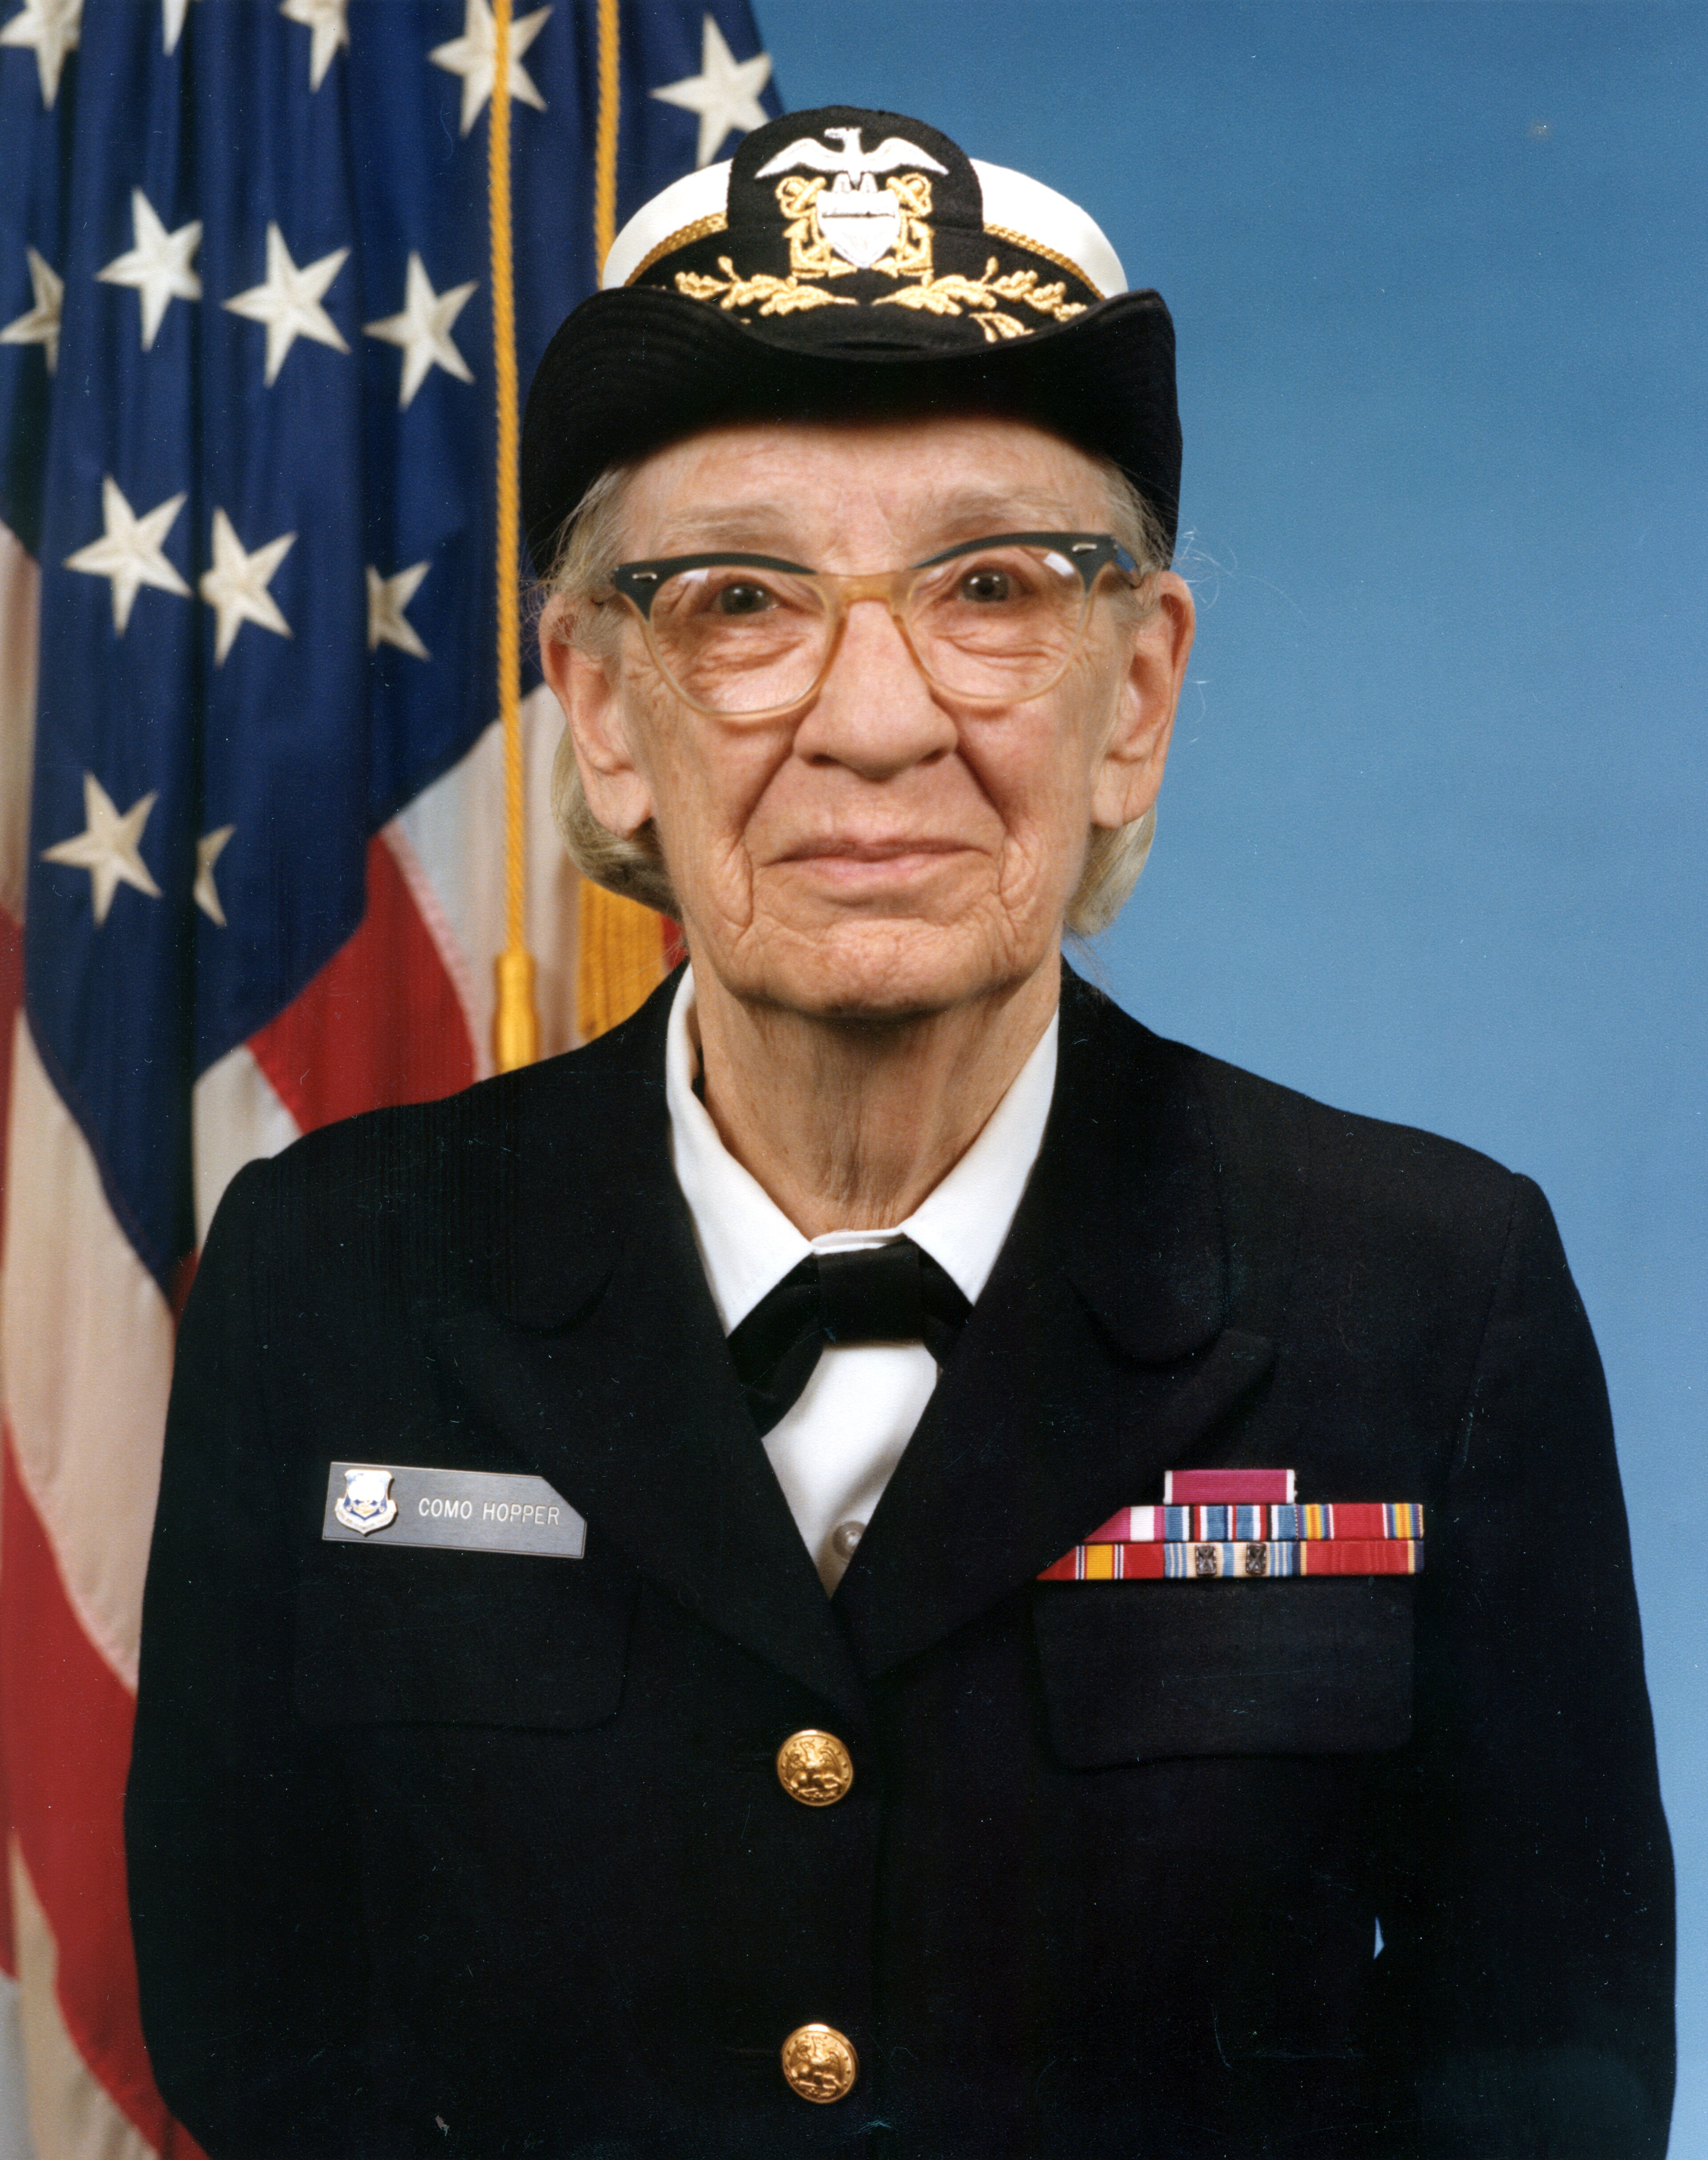
\includegraphics[height=4cm,keepaspectratio]{images/grace-hopper-2.jpg}\\
{\tiny\color{gktmuted}Grace Murray Hopper. Wikimedia Commons, public domain.}
\end{columns}
\end{frame}

% ============================================================
% 15 · CH7 ACCESS+AGENCY
% ============================================================
\begin{frame}{Machines Leave the Data Center}
\begin{columns}[T]
\column{0.55\textwidth}
\begin{itemize}
\item CHOC on the PDP-8 (1965): a new category of machine that \enquote{democratized access to computing.}
\item Engelbart's 1968 \enquote{Mother of All Demos} --- the mouse, hypertext, windows --- embodied his own philosophy: computers as \enquote{partners in human cognition and collaboration.}
\item Reaches classrooms, small businesses, university labs.
\end{itemize}
\chaptertag{\enquote{Time-Sharing and Interactive Computing}}
\column{0.45\textwidth}
\centering
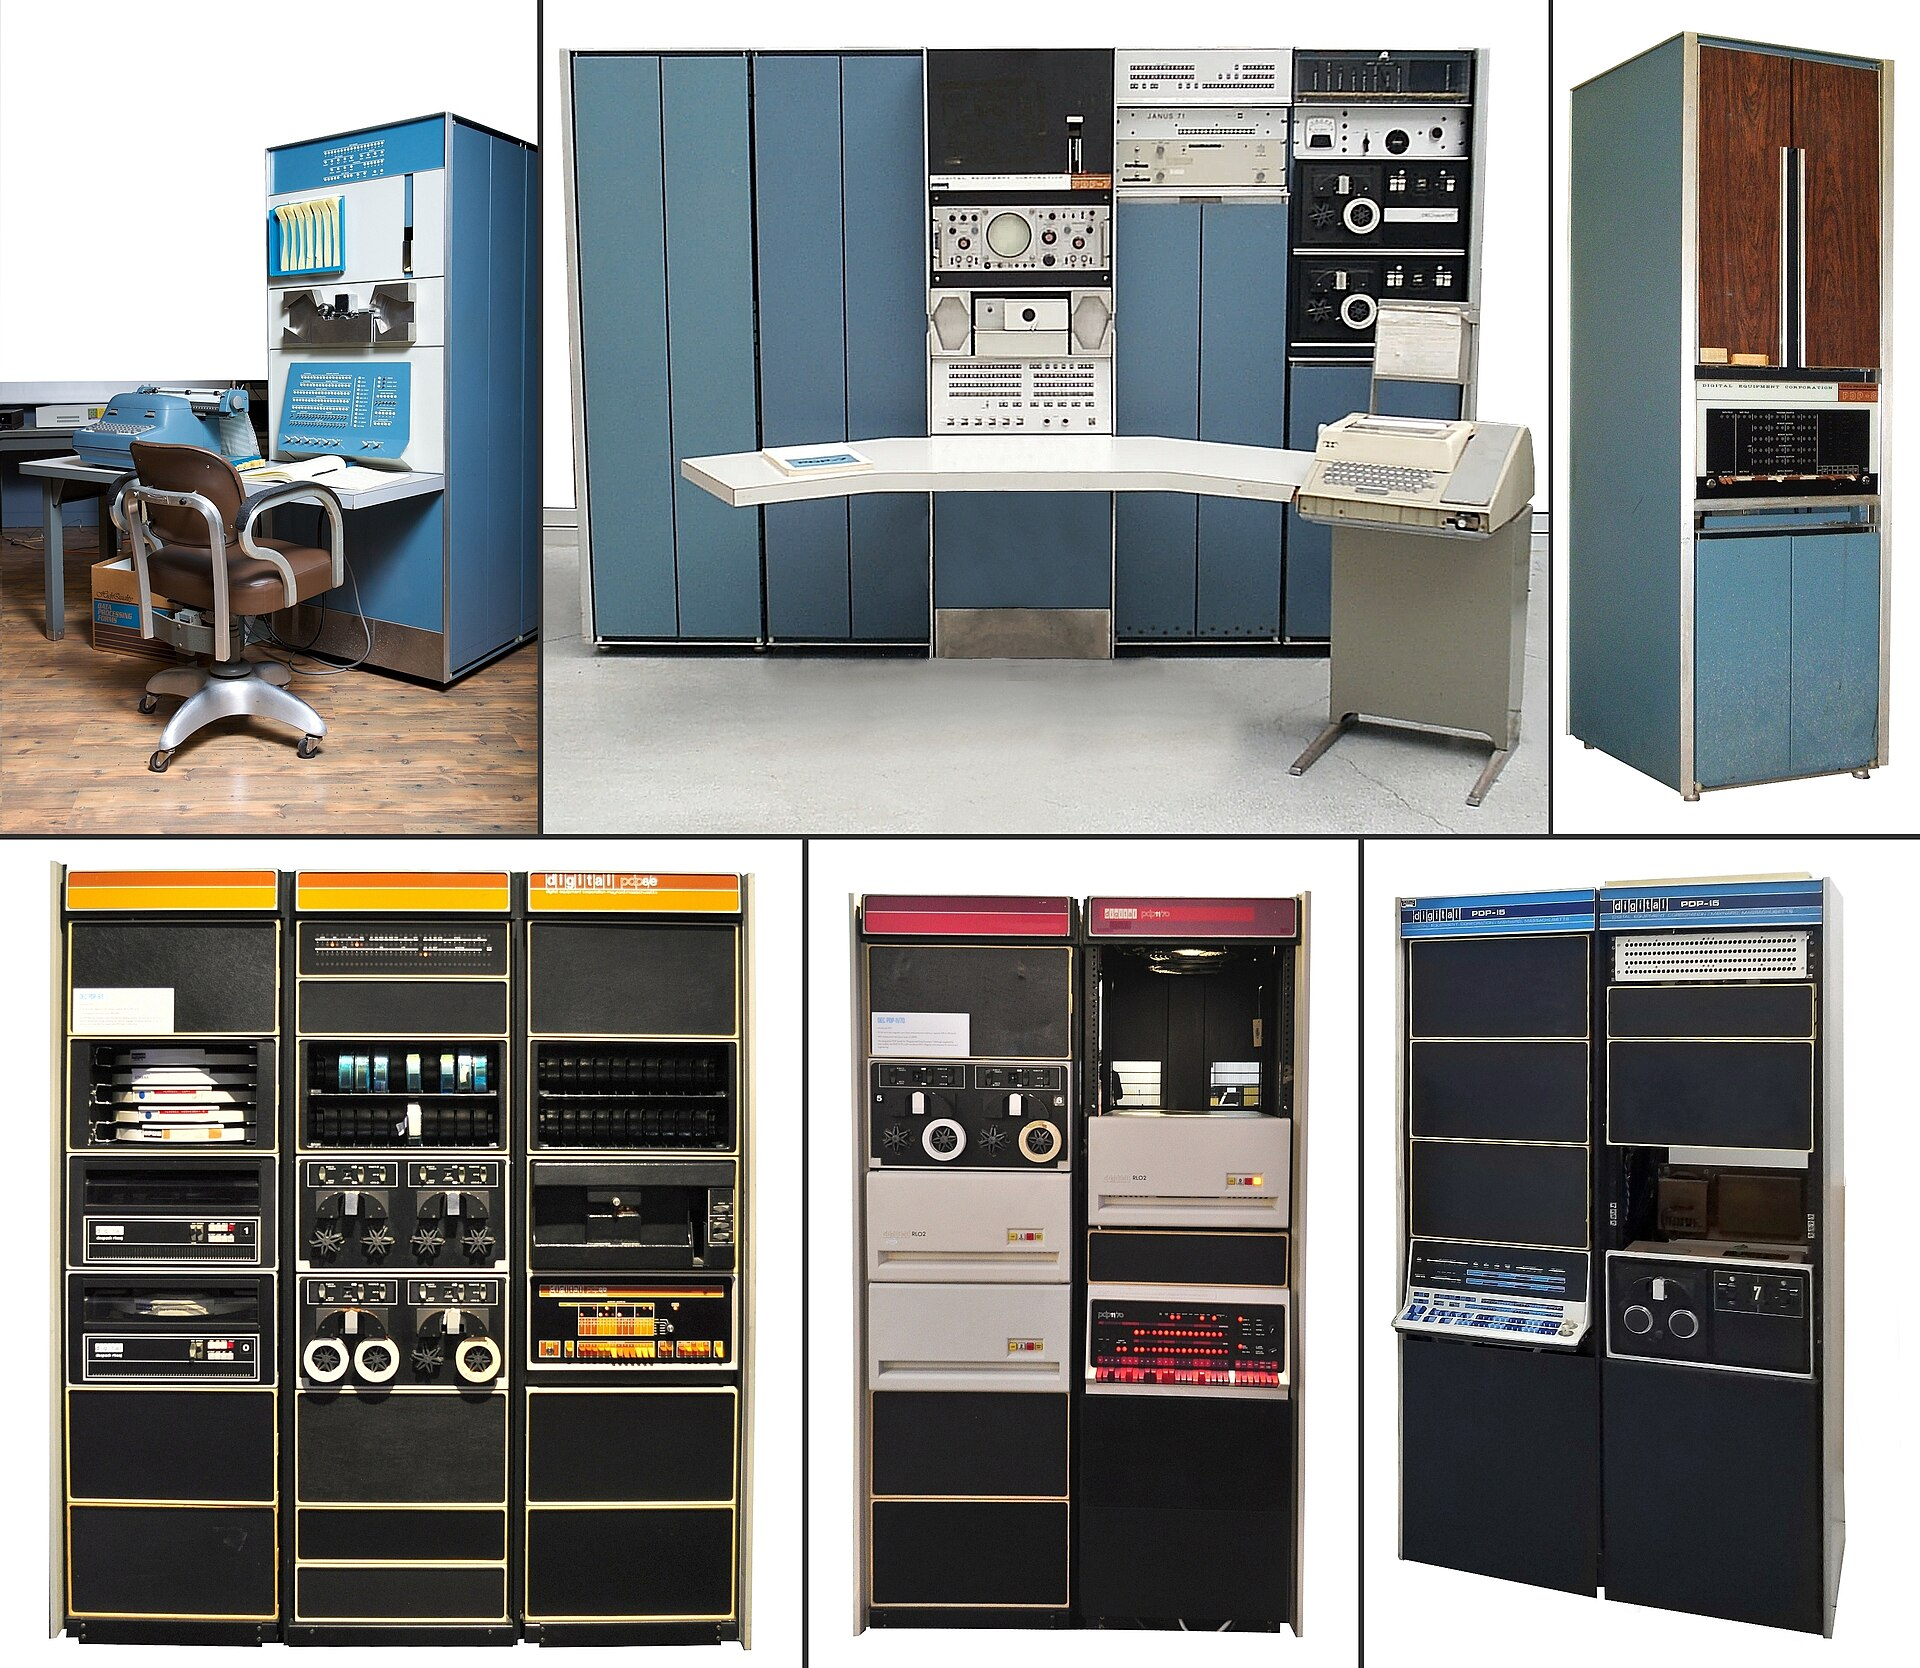
\includegraphics[height=4cm,keepaspectratio]{images/minicomputers.jpg}\\
{\tiny\color{gktmuted}DEC PDP-series minicomputers. Various photographers, Wikimedia Commons, CC BY-SA 4.0.}
\end{columns}
\end{frame}

% ============================================================
% 16 · CH8 ACCESS/LITERACY
% ============================================================
\begin{frame}{A Market Where None Had Existed}
\begin{columns}[T]
\column{0.55\textwidth}
\begin{itemize}
\item January 1975: the Altair 8800 on the cover of \emph{Popular Electronics}.
\item The Homebrew Computer Club --- hobbyists trading ideas freely.
\item CHOC: BASIC, Pascal, C \enquote{lowered barriers to entry, creating a broader base of technical literacy.}
\end{itemize}
\chaptertag{\enquote{Personal Computing as Promise}}
\column{0.45\textwidth}
\centering
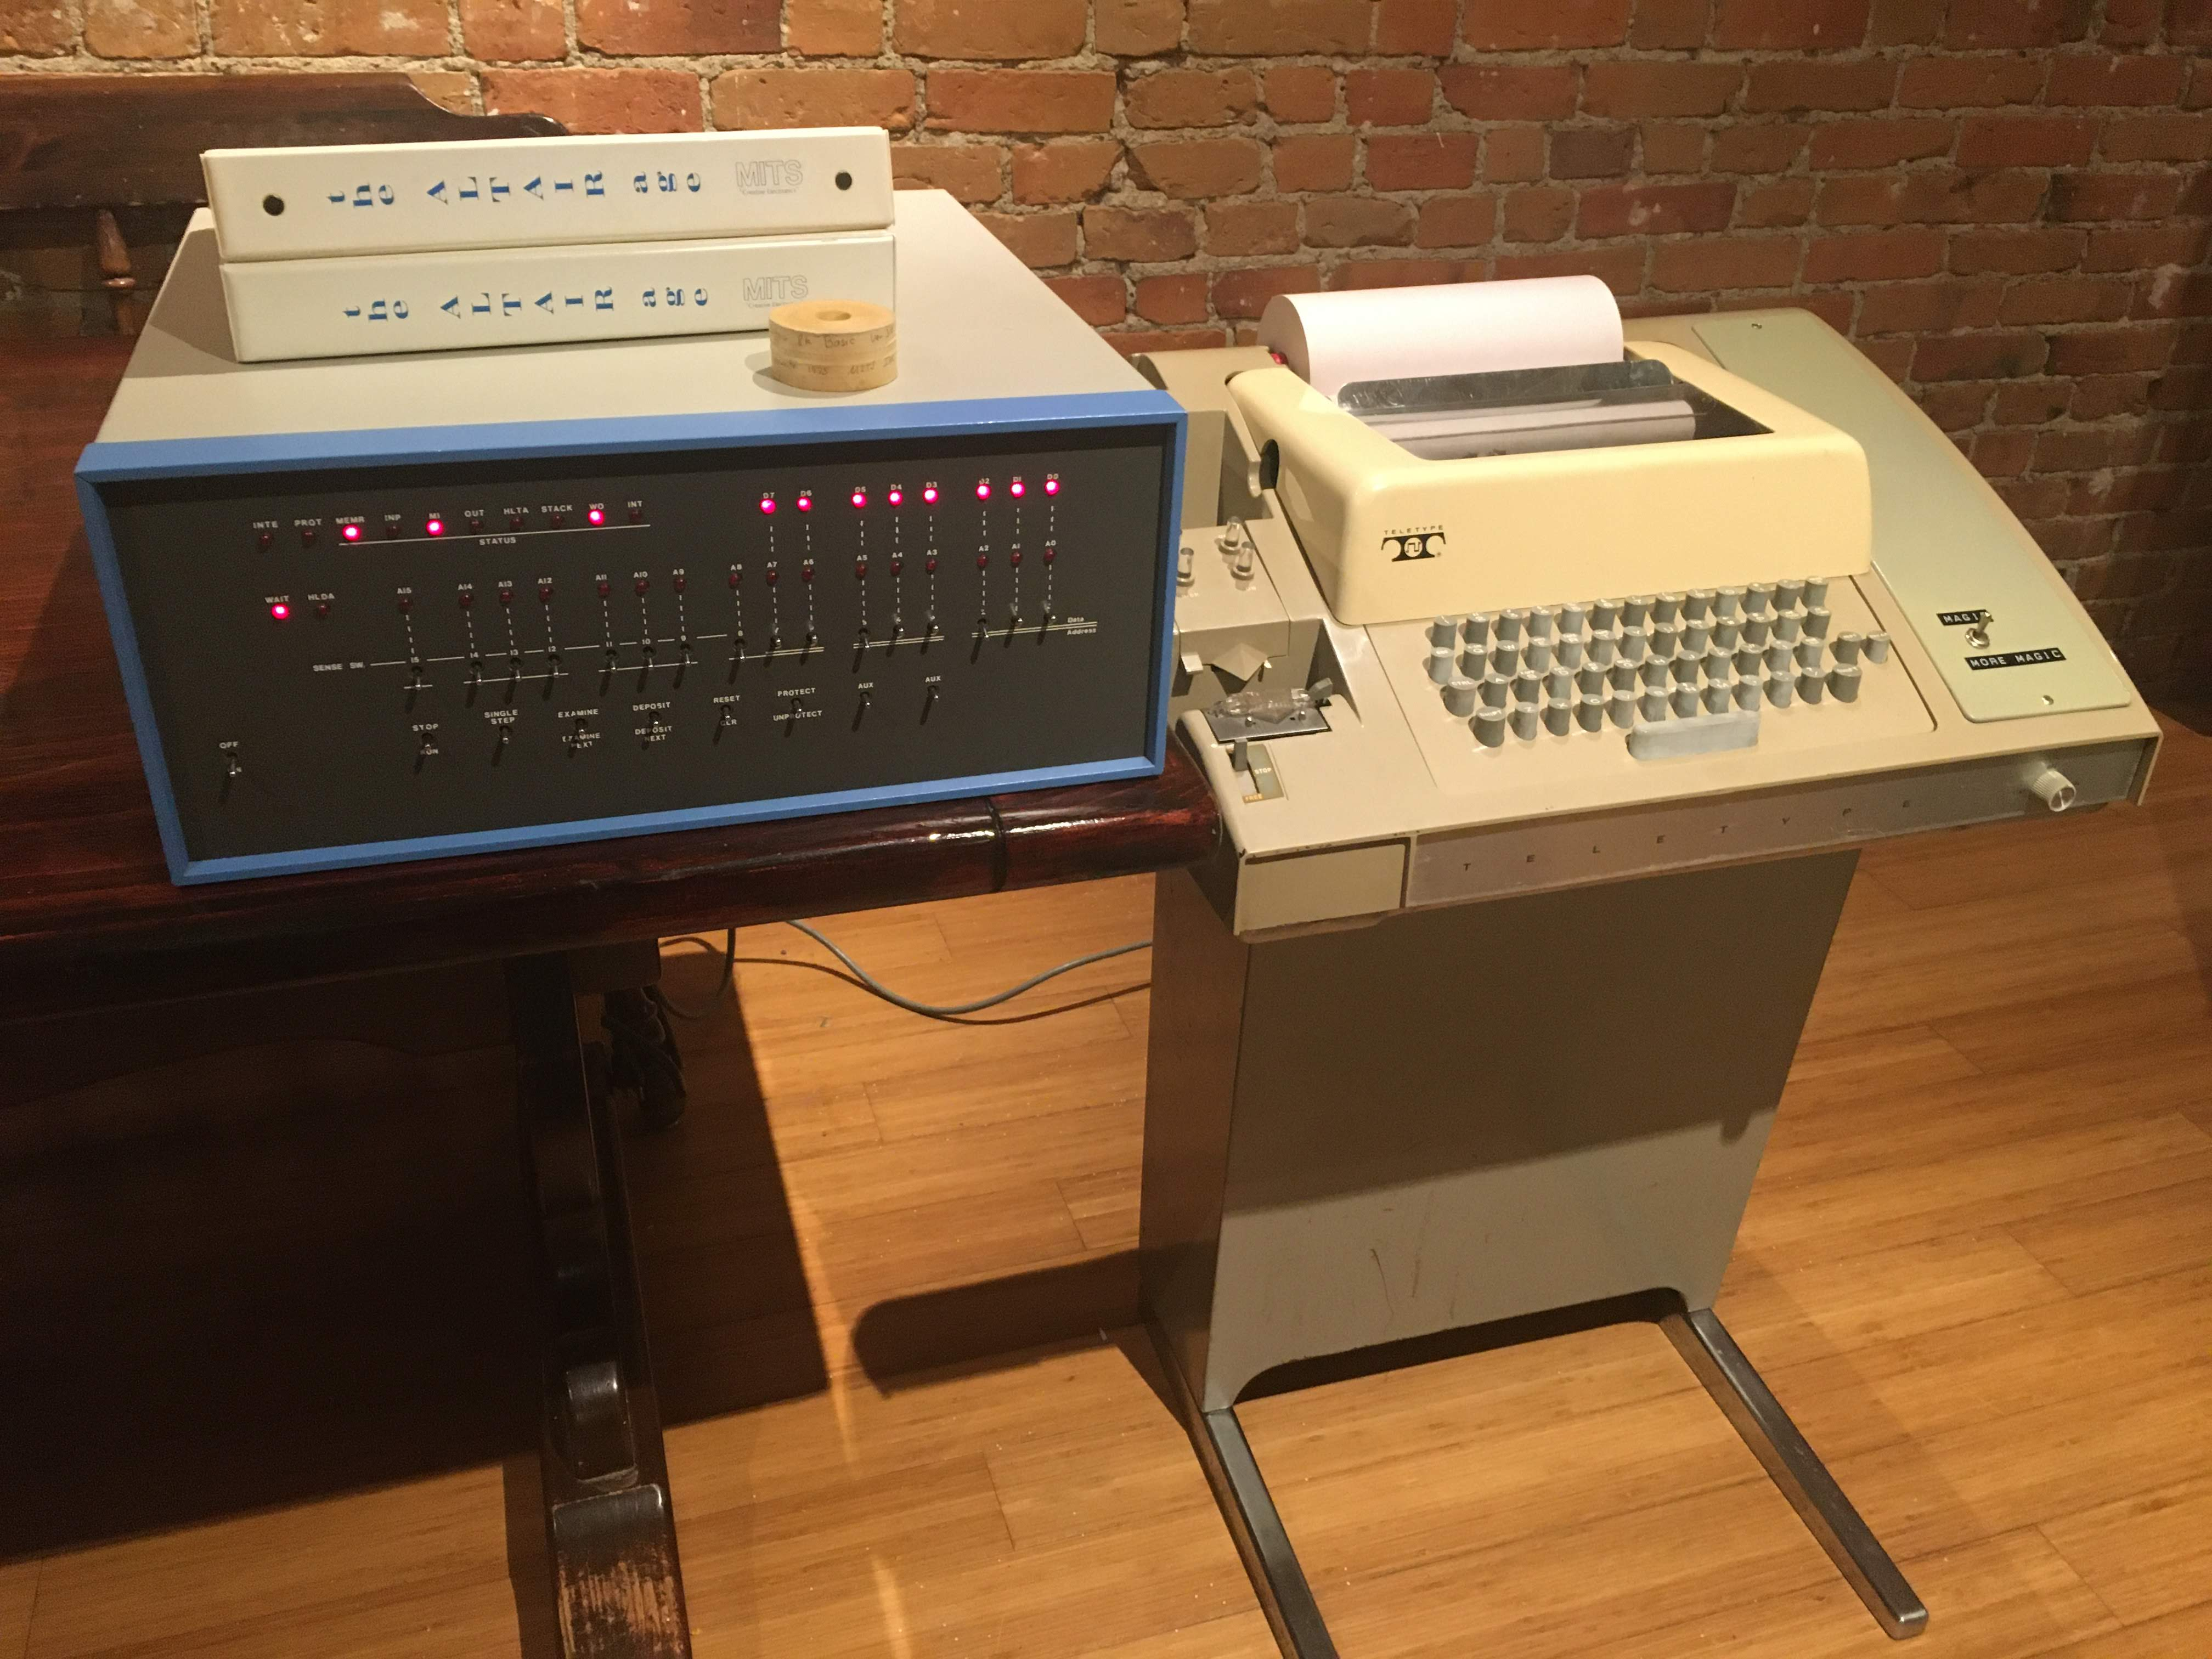
\includegraphics[height=4cm,keepaspectratio]{images/altair-8800-1.jpg}\\
{\tiny\color{gktmuted}Altair 8800 and Model 33 ASR Teletype. Tim Colegrove, Wikimedia Commons, CC BY-SA 4.0.}
\end{columns}
\end{frame}

% ============================================================
% 17 · CH9 ACCESS
% ============================================================
\begin{frame}{Elite Power vs. Democratized Access}
\begin{columns}[T]
\column{0.55\textwidth}
\begin{itemize}
\item CHOC's own contrast: supercomputers \enquote{embodied elite concentration of power}; personal computers \enquote{democratized access to computing.}
\item The Macintosh (1984) makes the graphical interface --- Engelbart's lineage --- a consumer product.
\item Two machines, same decade, opposite answers to \enquote{who gets to compute.}
\end{itemize}
\chaptertag{\enquote{Personal Computers, Interfaces, and Early Networks}}
\column{0.45\textwidth}
\centering
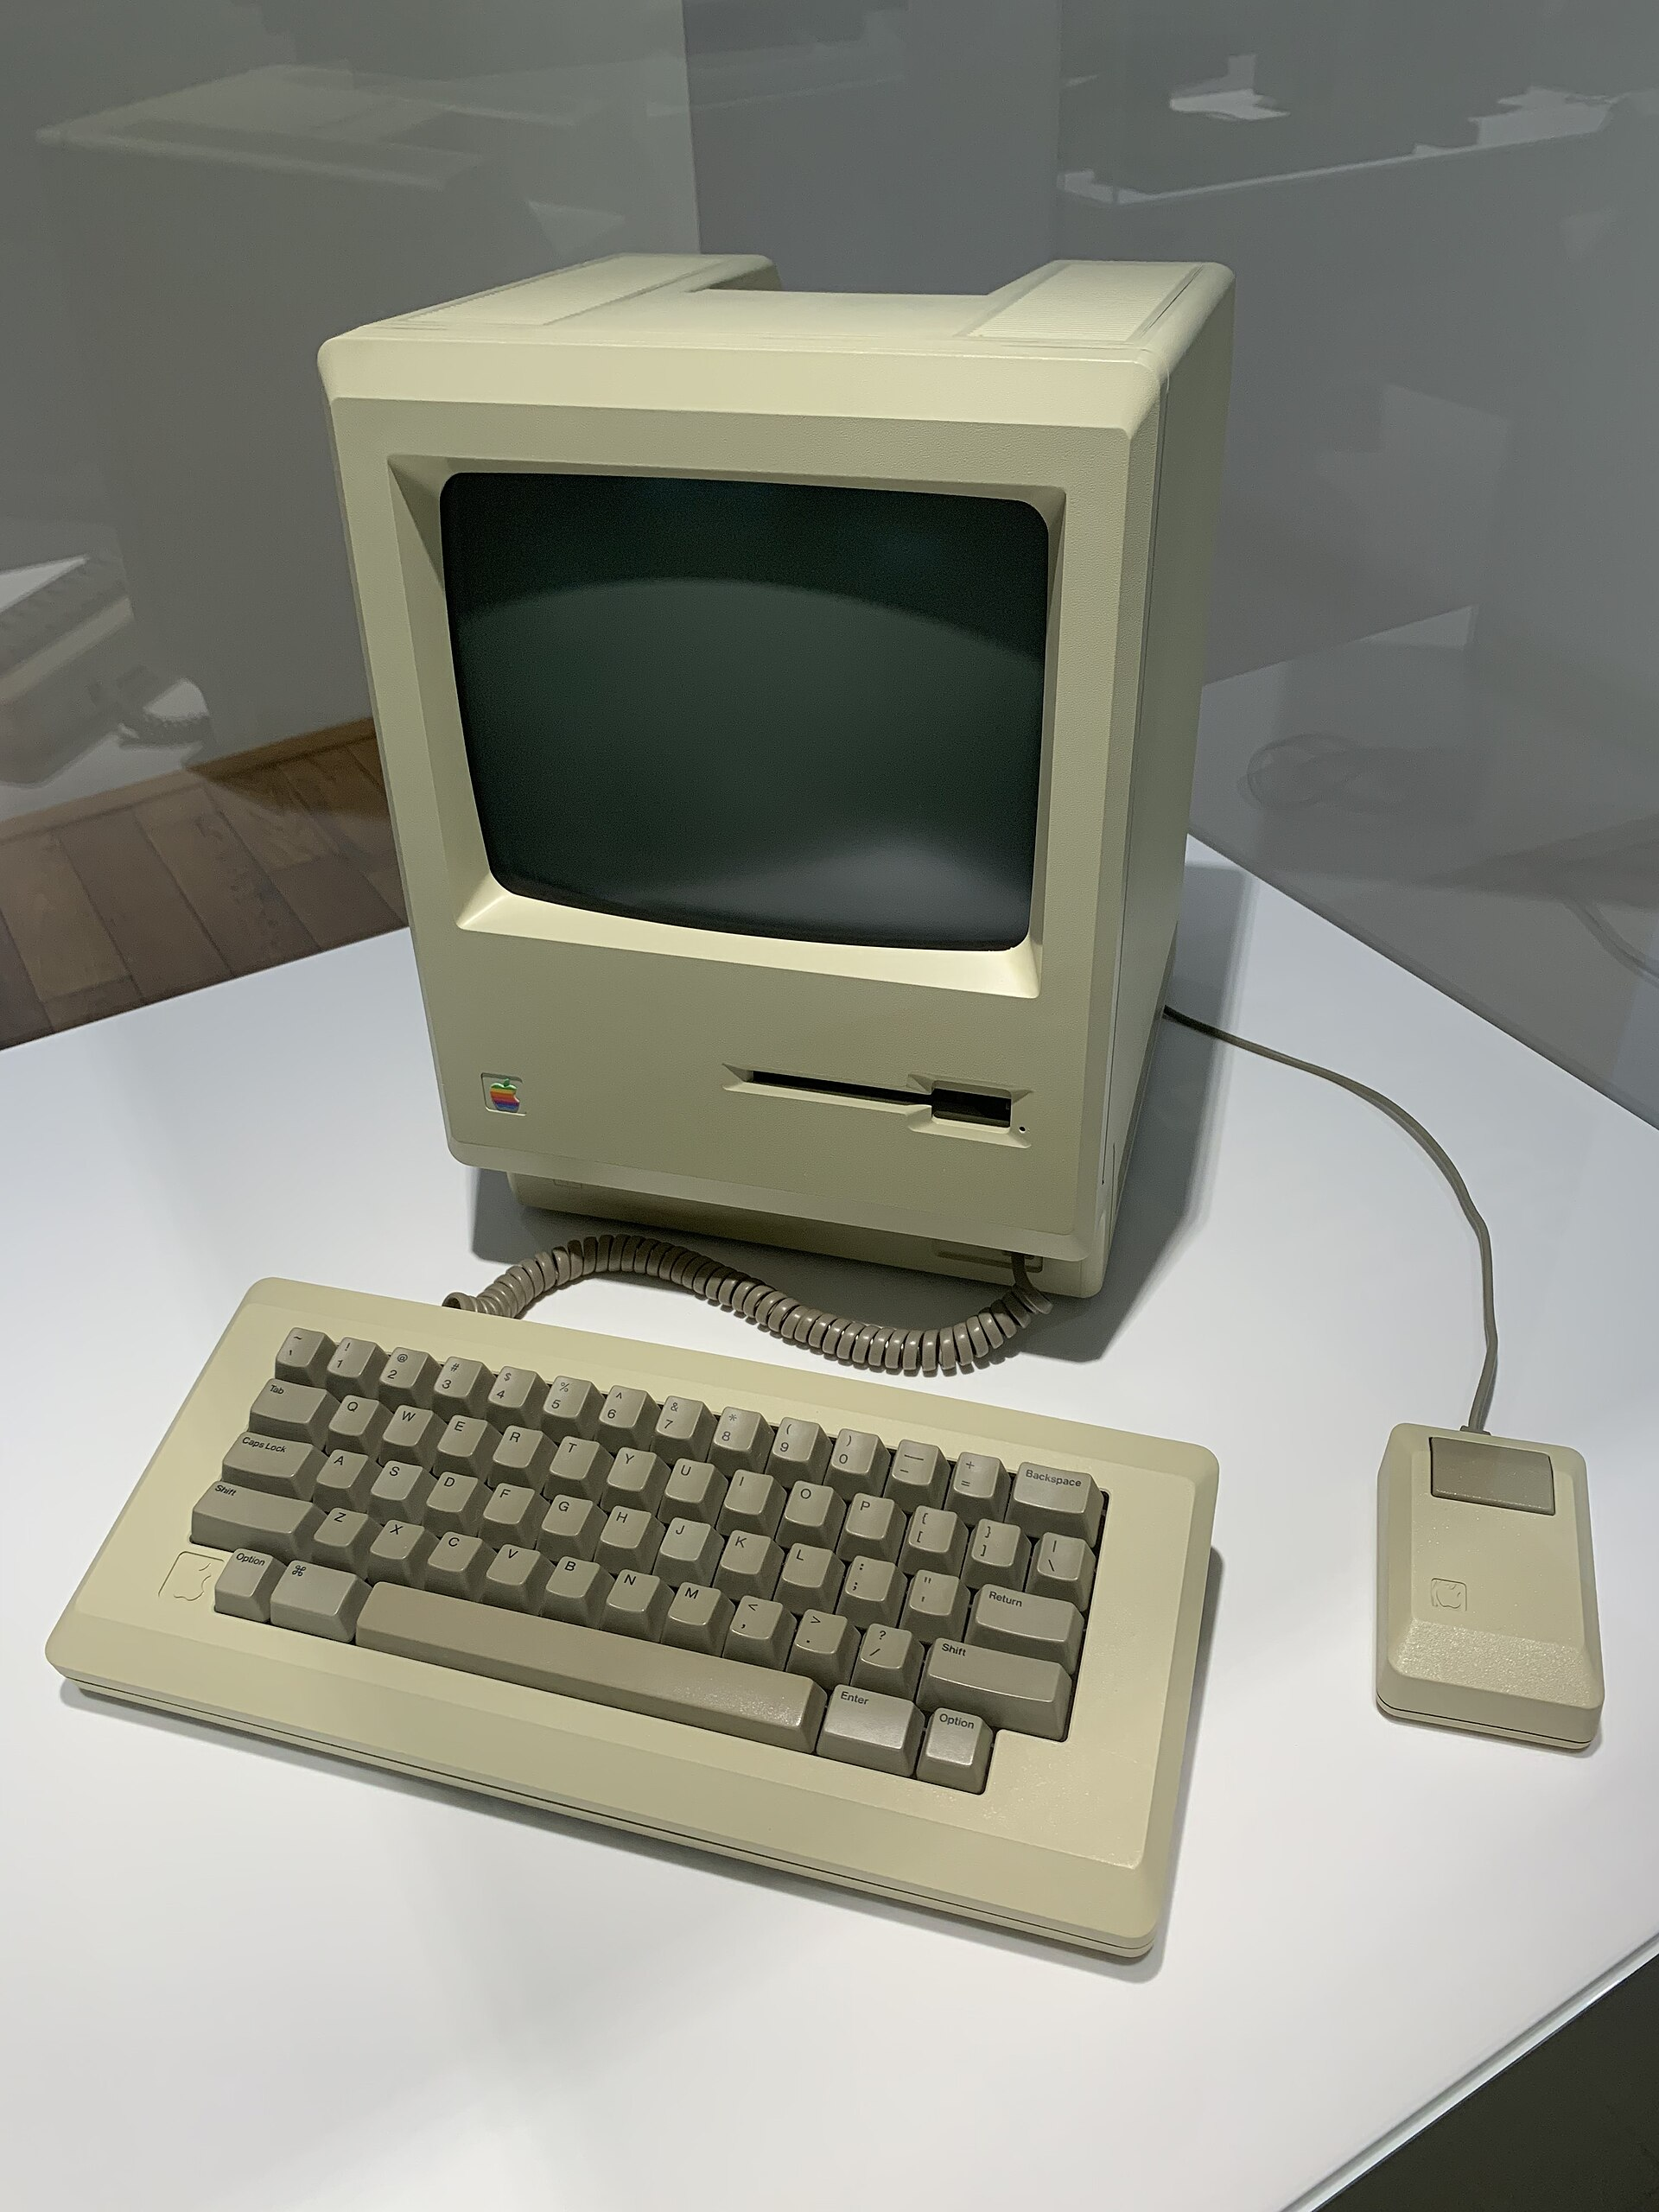
\includegraphics[height=4cm,keepaspectratio]{images/apple-mac.jpg}\\
{\tiny\color{gktmuted}Original Apple Macintosh, Apple Museum Prague. Beno\^{\i}t Prieur, Wikimedia Commons, CC0.}
\end{columns}
\end{frame}

% ============================================================
% 18 · CH9 AGENCY
% ============================================================
\begin{frame}{Freedom From the Radio Playlist}
\begin{columns}[T]
\column{0.55\textwidth}
\begin{itemize}
\item The Walkman (1979): the first portable cassette player, small enough to carry everywhere.
\item Critics called it antisocial; CHOC says users \enquote{embraced it as autonomy.}
\item Elsewhere: \enquote{For the first time, media moved with the user, not the other way around.}
\end{itemize}
\chaptertag{\enquote{Culture: Playback Media and Electronic Spectacle}}
\column{0.45\textwidth}
\centering
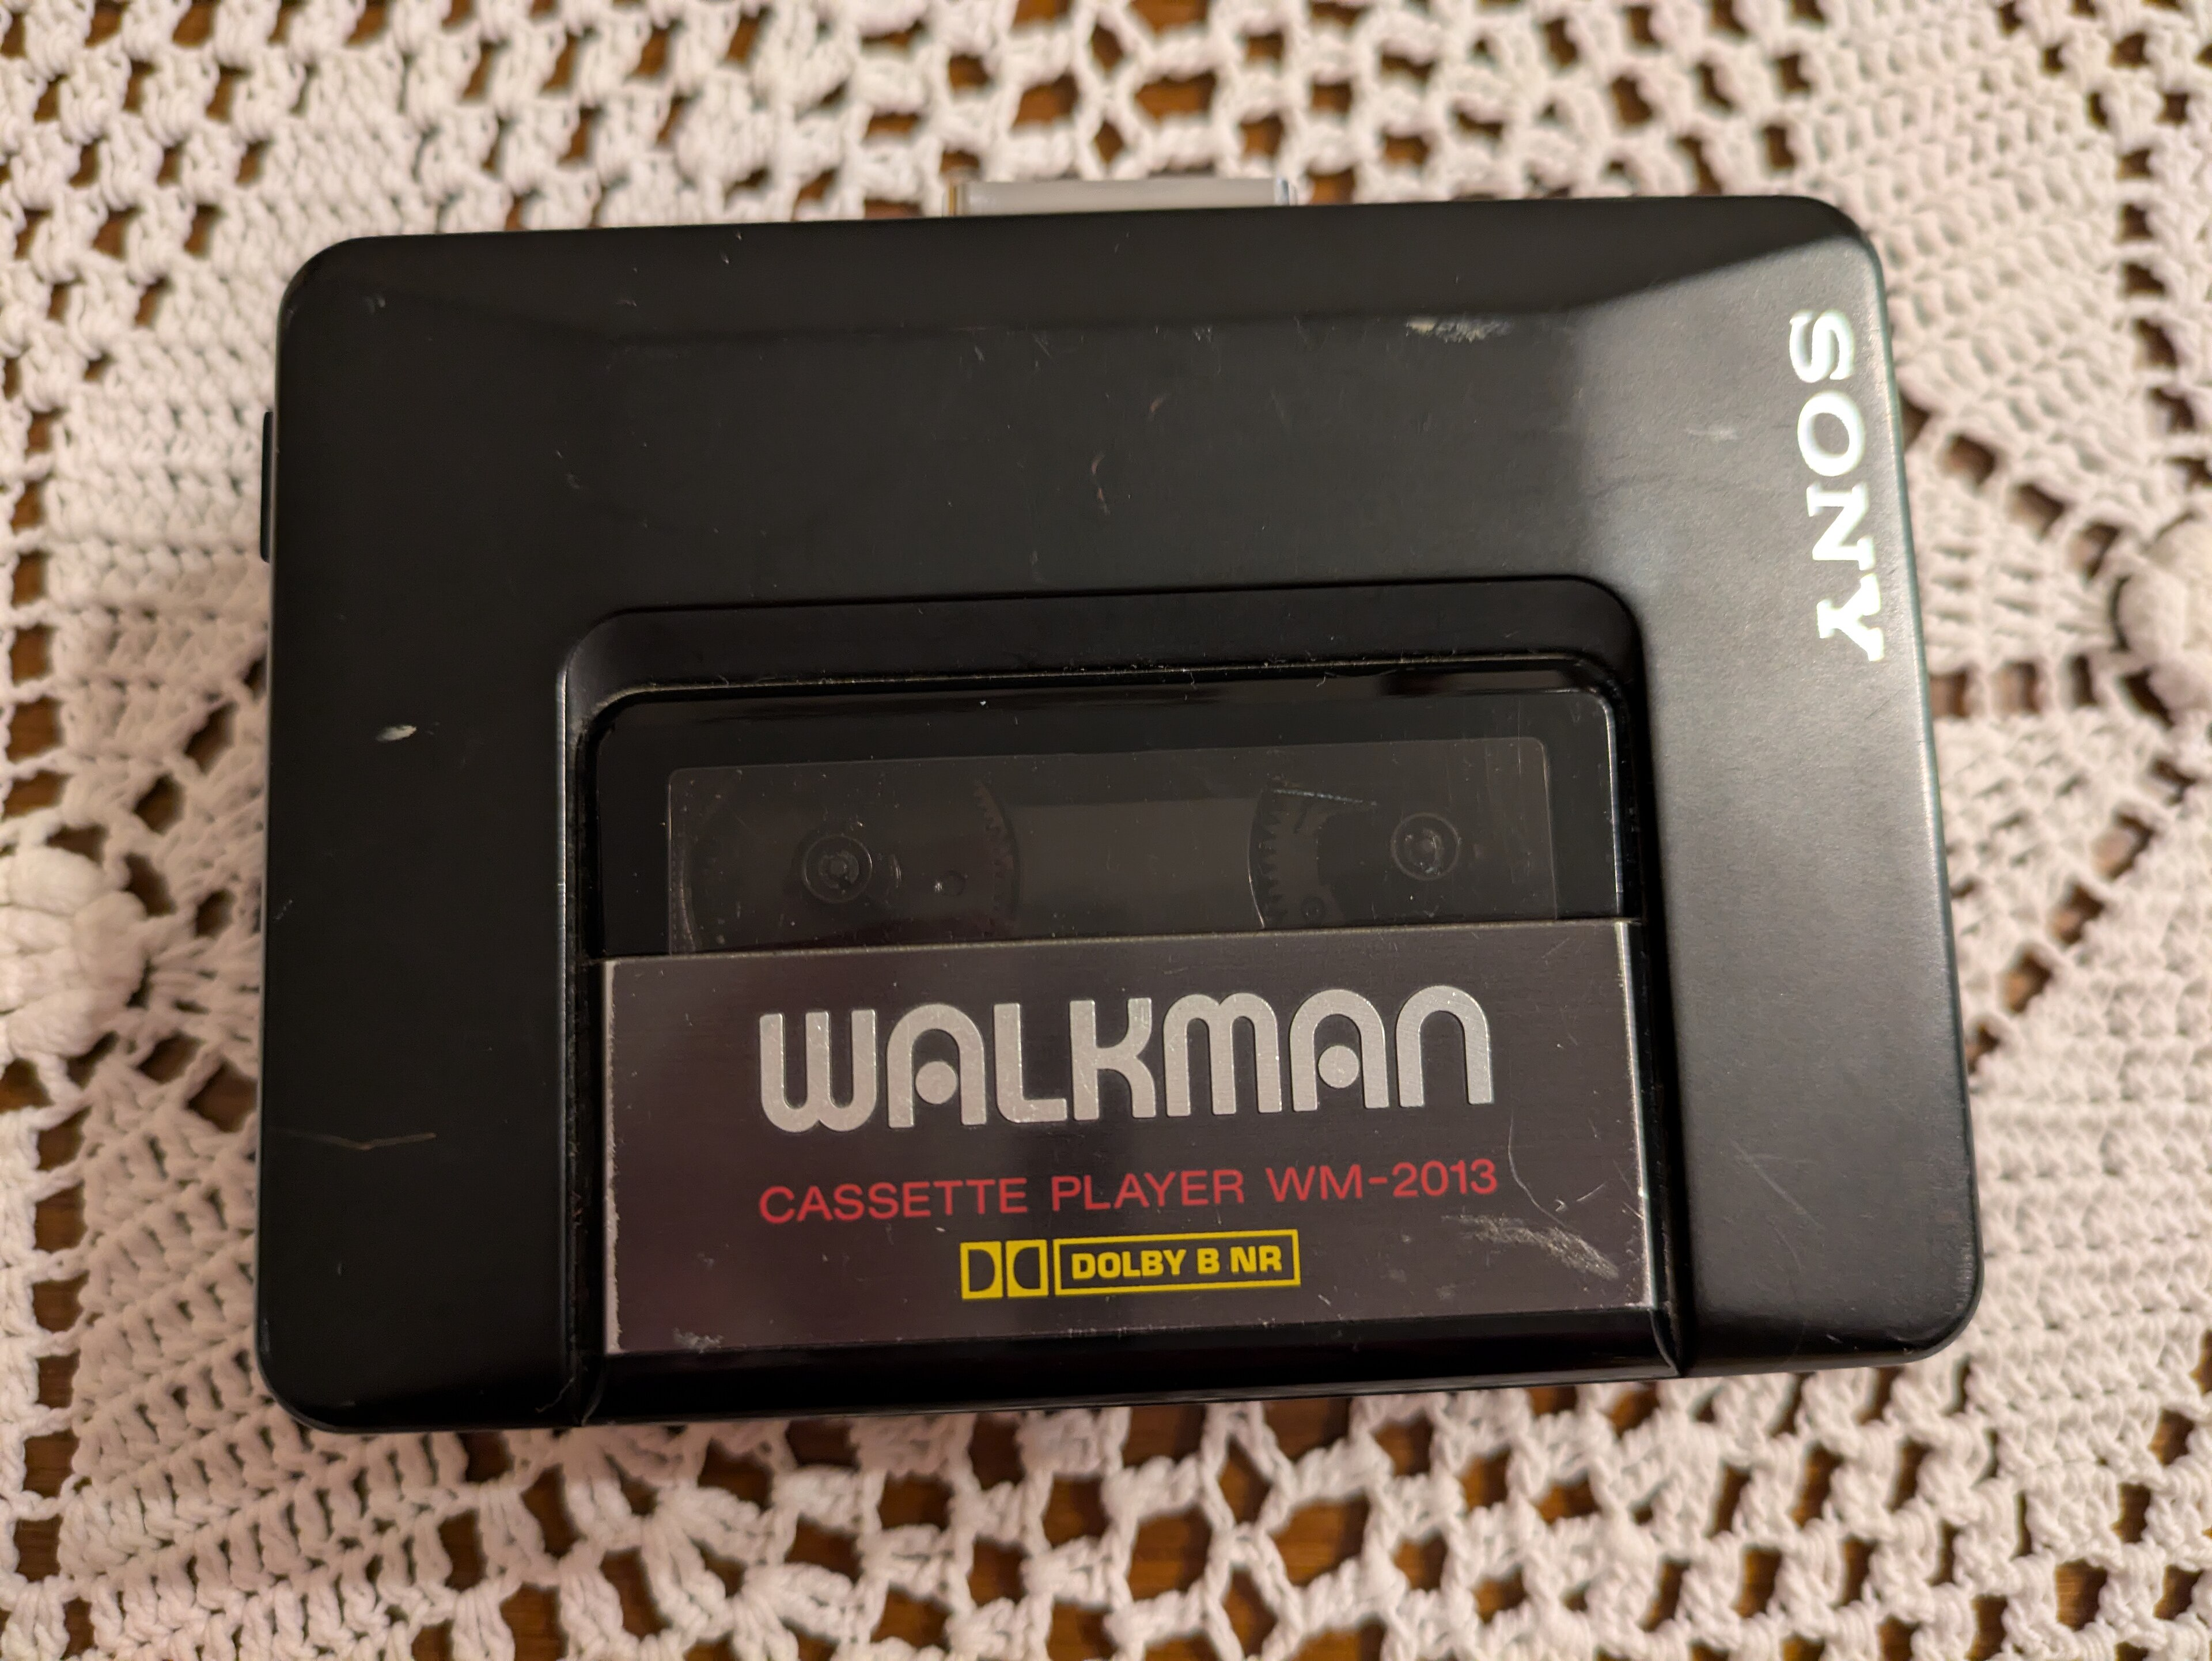
\includegraphics[height=4cm,keepaspectratio]{images/walkman.jpg}\\
{\tiny\color{gktmuted}Original Sony Walkman TPS-L2. Binarysequence, Wikimedia Commons, CC BY-SA 4.0.}
\end{columns}
\end{frame}

% ============================================================
% 19 · CH10 ACCESS
% ============================================================
\begin{frame}{The Web Becomes Point-and-Click}
\begin{columns}[T]
\column{0.55\textwidth}
\begin{itemize}
\item 1993: NCSA Mosaic --- the first browser to combine graphics and text in one window.
\item CHOC's assessment: a turning point \enquote{as consequential as the IBM PC in 1981 or Windows 95 in 1995.}
\item Redefined what it meant to use a computer at all.
\end{itemize}
\chaptertag{\enquote{Browsers, Services, and the New Economy}}
\column{0.45\textwidth}
\centering
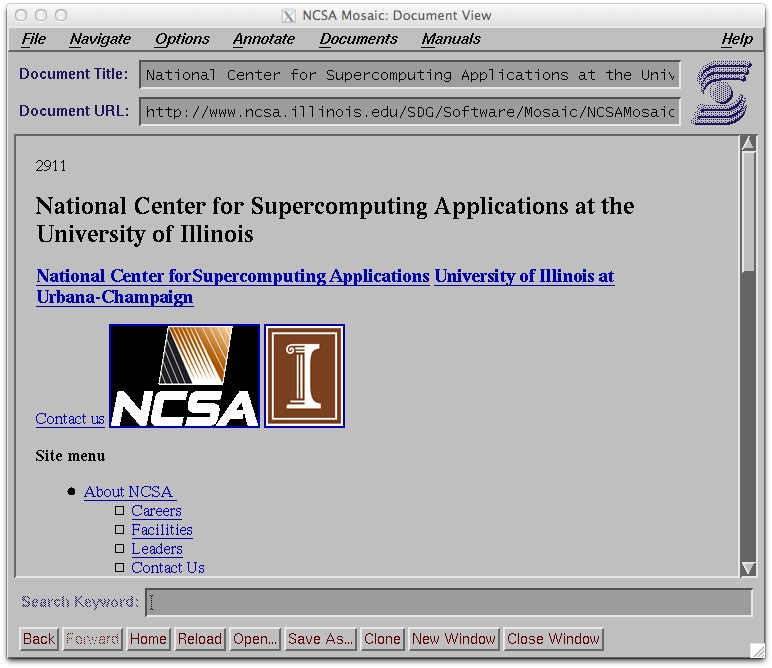
\includegraphics[height=4cm,keepaspectratio]{images/mosaic.png}\\
{\tiny\color{gktmuted}NCSA Mosaic browser screenshot. Charles Severance, Wikimedia Commons, CC0.}
\end{columns}
\end{frame}

% ============================================================
% 20 · CH10 ACCOUNTABILITY
% ============================================================
\begin{frame}{The Browser Wars}
\begin{columns}[T]
\column{0.55\textwidth}
\begin{itemize}
\item Netscape Navigator (1994) captures the lion's share of Web traffic; 1995 IPO fuels the dot-com boom.
\item Microsoft bundles Internet Explorer into Windows --- 1998 DOJ antitrust suit follows.
\item Platform accountability disputes did not begin with social media.
\end{itemize}
\chaptertag{\enquote{Browsers, Services, and the New Economy}}
\column{0.45\textwidth}
\centering
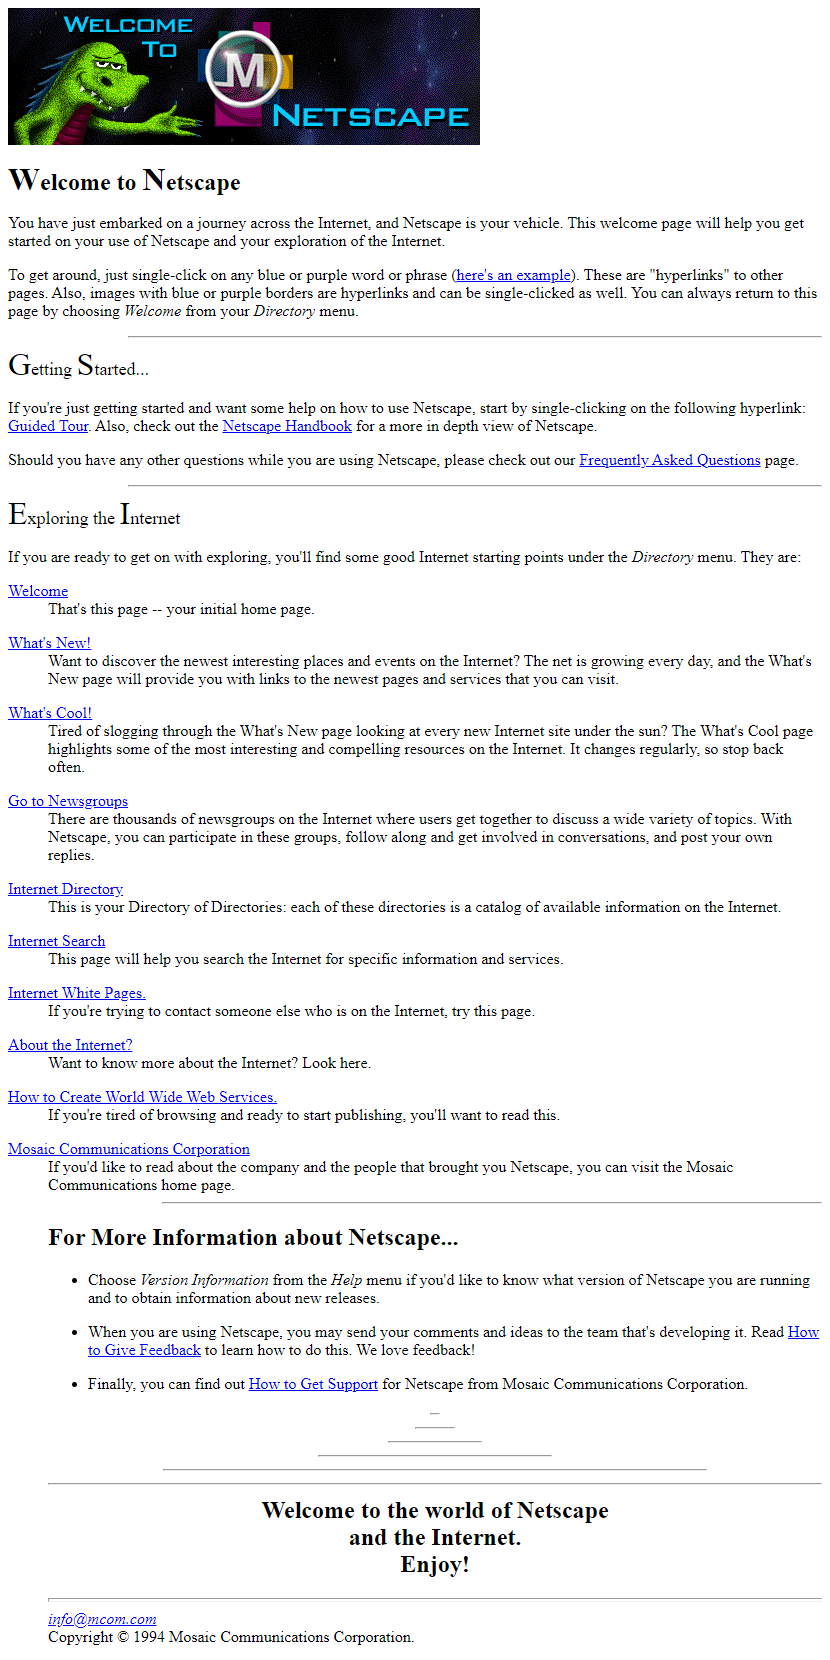
\includegraphics[height=4cm,keepaspectratio]{images/netscape-1994.png}\\
{\tiny\color{gktmuted}Screenshot of the Netscape website in 1994. Web Design Museum, used with permission.}
\end{columns}
\end{frame}

% ============================================================
% 21 · CH11 ACCOUNTABILITY
% ============================================================
\begin{frame}{The Networked Society's Janus Face}
\begin{columns}[T]
\column{0.55\textwidth}
\begin{itemize}
\item WikiLeaks/Manning (2010) exposes what governments hide.
\item The Patriot Act, NSA, and warrantless wiretapping expand what governments see.
\item CHOC's verdict: \enquote{the networked society revealed its Janus face\ldots{} transparency and secrecy, empowerment and control, were no longer opposites but entangled dynamics of the same infrastructures.}
\end{itemize}
\chaptertag{\enquote{Web 2.0, Smartphones, and the Cloud}}
\column{0.45\textwidth}
\centering
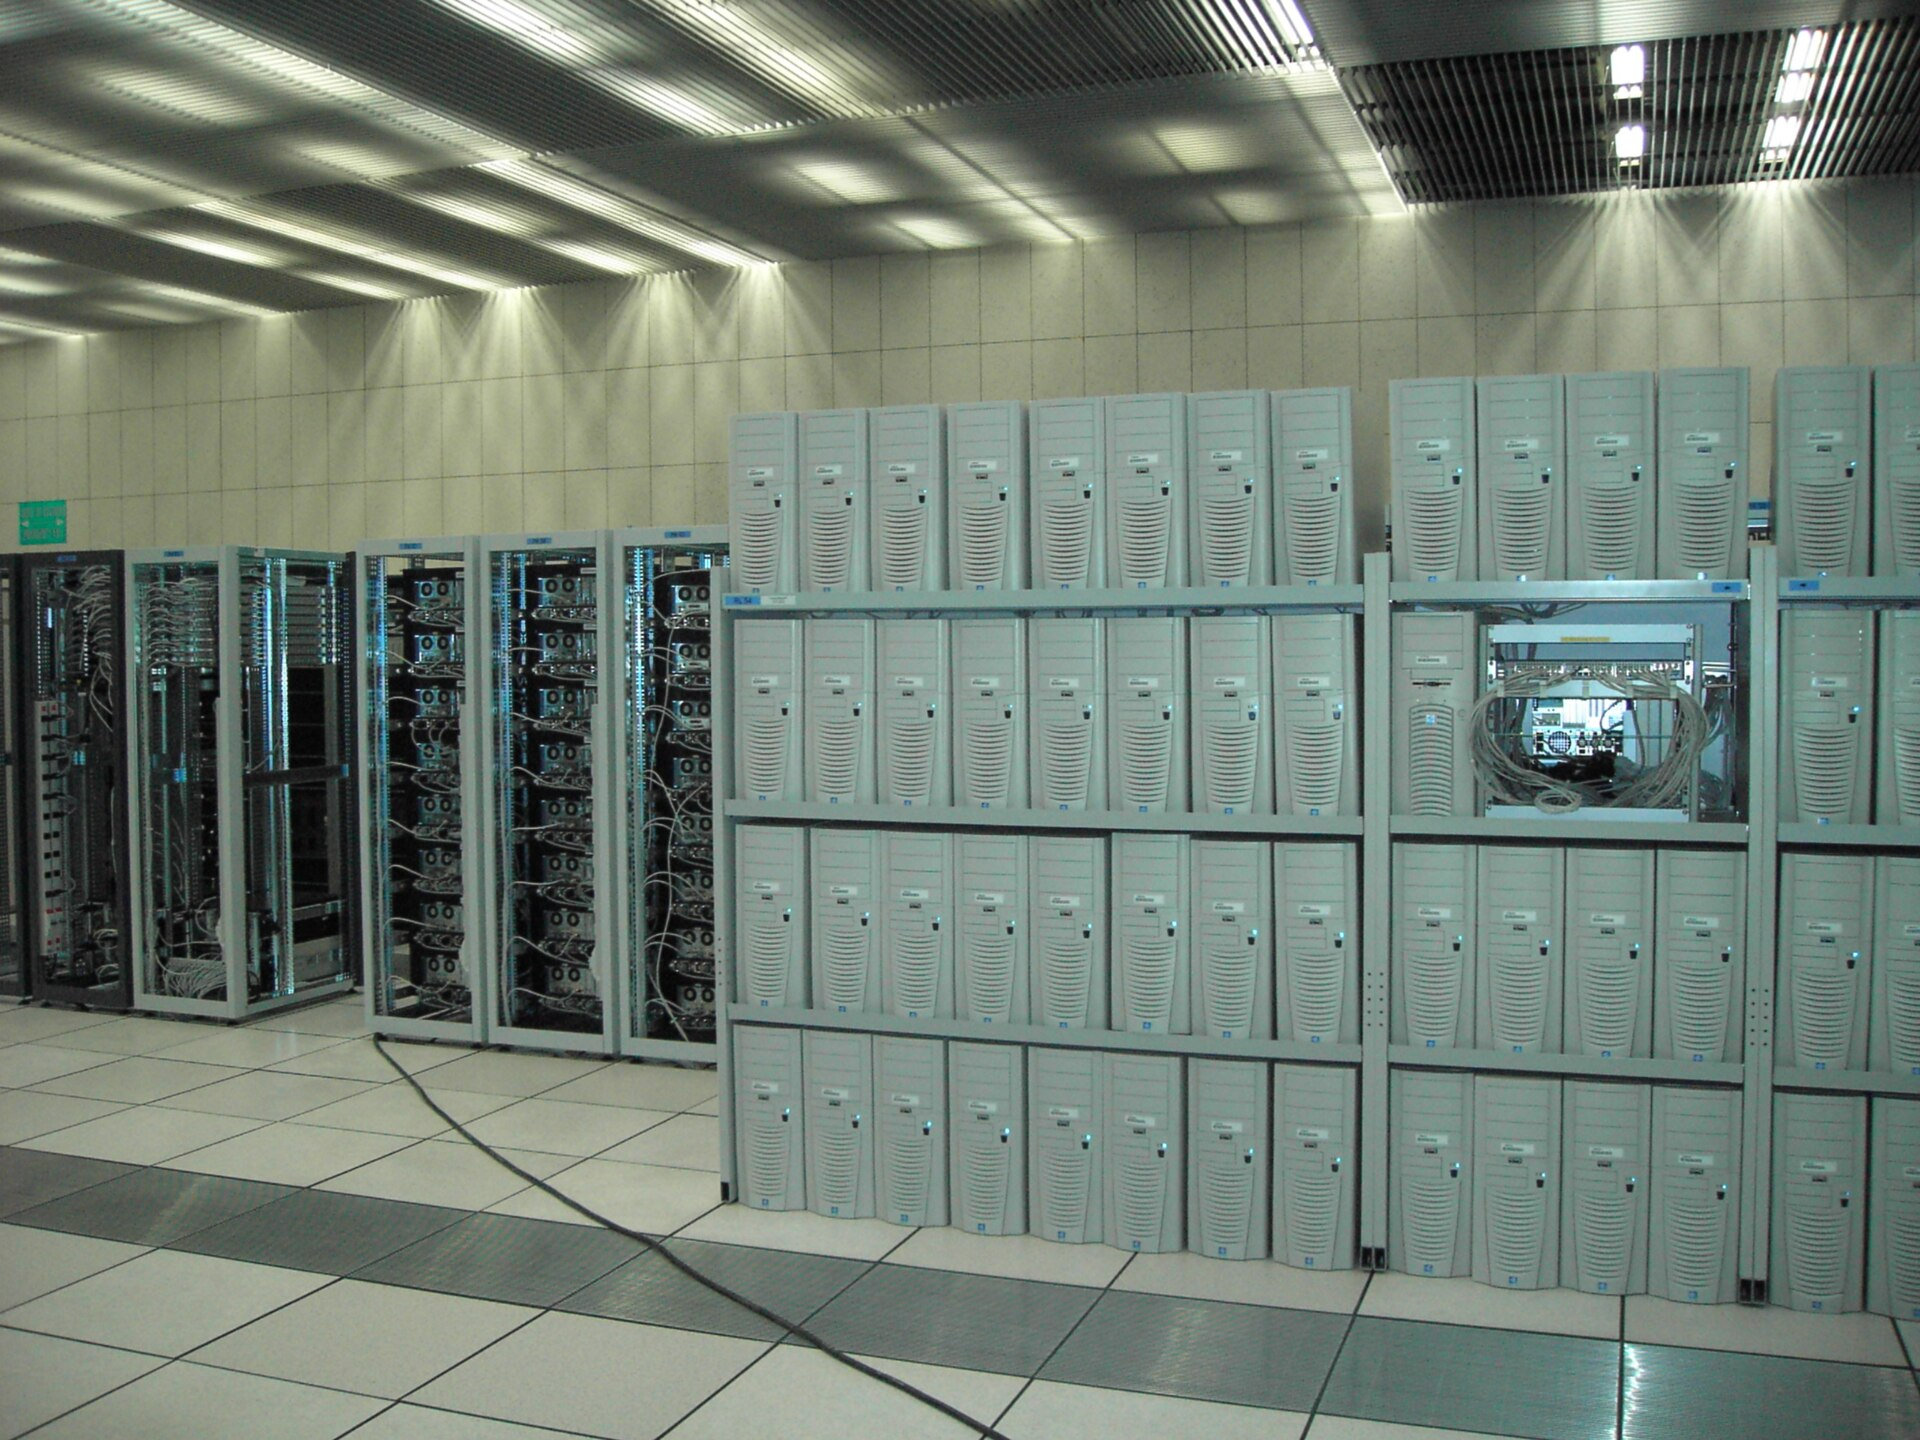
\includegraphics[height=4cm,keepaspectratio]{images/server-farm.jpg}\\
{\tiny\color{gktmuted}NASA computer server farm. Wikimedia Commons, public domain.}
\end{columns}
\end{frame}

% ============================================================
% 22 · CH11 ACCESS
% ============================================================
\begin{frame}{The Convergence Artifact}
\begin{columns}[T]
\column{0.55\textwidth}
\begin{itemize}
\item The iPhone (2007): camera, browser, phone, and platform in one object.
\item Castells' \enquote{network society} stops being theory and becomes lived condition.
\item Smartphones become the primary access point to computing worldwide.
\end{itemize}
\chaptertag{\enquote{Web 2.0, Smartphones, and the Cloud}}
\column{0.45\textwidth}
\centering
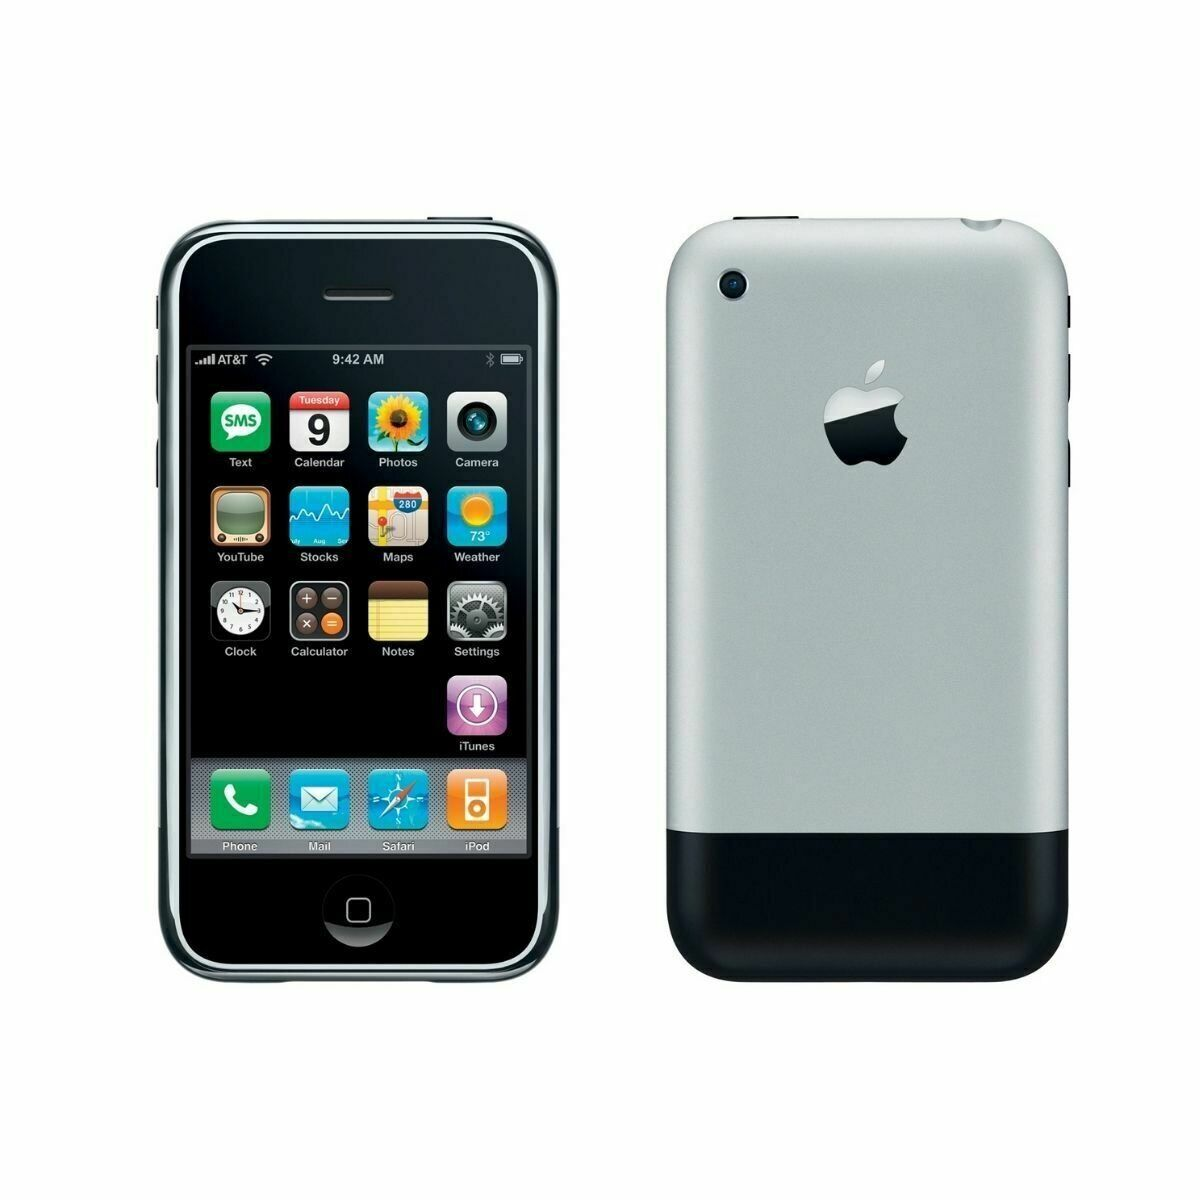
\includegraphics[height=4cm,keepaspectratio]{images/original-apple-iphone.jpg}\\
{\tiny\color{gktmuted}iPhone (2007). Avicente05, Wikimedia Commons, CC BY-SA 4.0.}
\end{columns}
\end{frame}

% ============================================================
% 22a · MEMEX/WORLD BRAIN THROUGHLINE
% ============================================================
\begin{frame}{A Library That Was Always Coming}
\begin{itemize}
\item 1945: Vannevar Bush's essay \enquote{As We May Think} imagines the memex --- a device for augmenting human memory and association. No AI involved; the idea is 80 years old.
\item CHOC returns to this vision three separate times --- at the CD-ROM, the Web, and Wikipedia --- each a partial realization of the same 1945 idea.
\item CHOC's own verdict: singularity \enquote{no longer described a hypothetical future in which artificial intelligence exceeded human cognition, but a present reality in which human culture and digital systems had become inseparable.}
\end{itemize}
\chaptertag{\enquote{The Memex/World Brain Throughline}}
\end{frame}

% ============================================================
% 23 · CH12 AUTOMATION
% ============================================================
\begin{frame}{The Edge of Automation, Before Anyone Called It AI}
\begin{columns}[T]
\column{0.55\textwidth}
\begin{itemize}
\item CHOC's account: \enquote{datafication} of ordinary behavior --- clicks, GPS traces, likes --- becomes a monetized reservoir; critics (elsewhere) called it \enquote{surveillance capitalism.}
\item 2012: deep learning classifies images with unprecedented accuracy.
\item By mid-decade, CHOC argues, algorithms were \enquote{silently shaping cultural consumption\ldots{} They did not merely respond to human choices; they guided them.}
\end{itemize}
\chaptertag{\enquote{Data, AI, and the Edge of Automation}}
\column{0.45\textwidth}
\centering
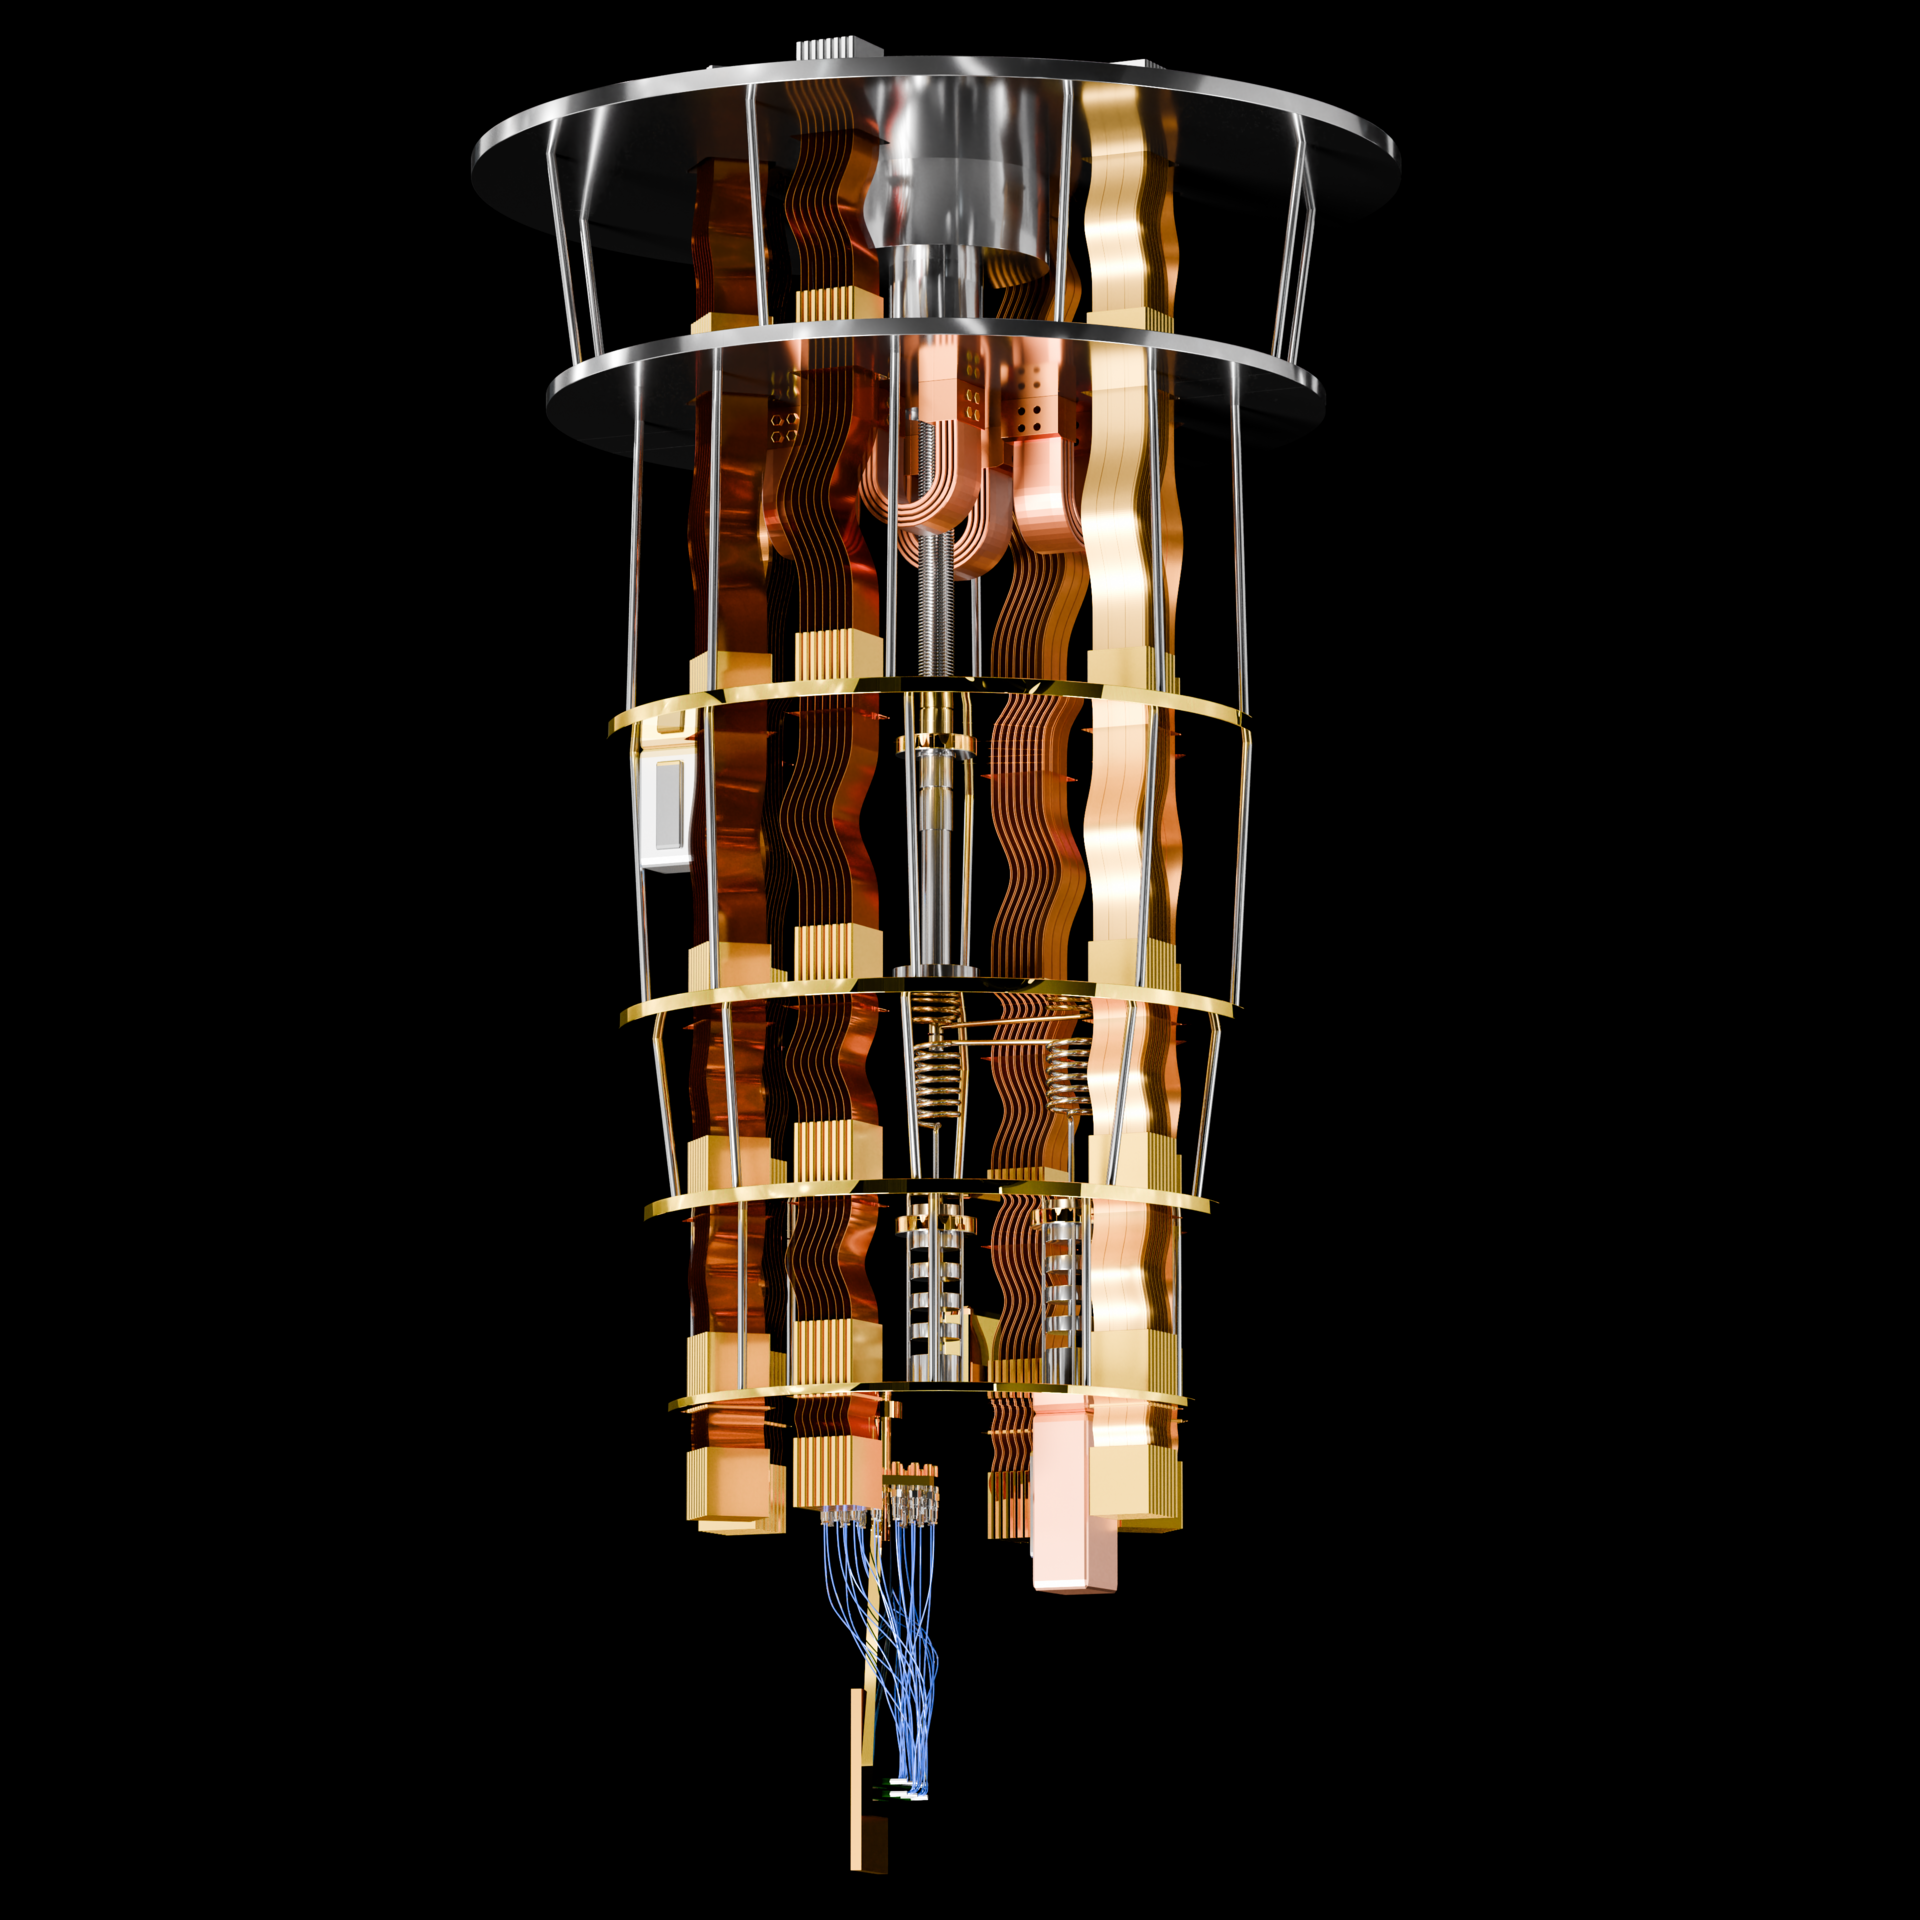
\includegraphics[height=4cm,keepaspectratio]{images/quantum-computer.png}\\
{\tiny\color{gktmuted}Quantum computer. Wikimedia Commons, public domain.}
\end{columns}
\end{frame}

% ============================================================
% 24 · CH12 ACCESS+LABOR
% ============================================================
\begin{frame}{Global in Reach, Fragmented in Practice}
\begin{columns}[T]
\column{0.55\textwidth}
\begin{itemize}
\item Four models of the 2010s network: U.S. ad-driven, EU regulatory, Chinese platform-state, Global South mobile-leapfrogging (M-Pesa, Jio).
\item CHOC's paradox: \enquote{communications in the 2010s were global in reach but fragmented in practice.}
\item On the creator economy, CHOC: influencer labor was \enquote{both artistic performance and data-driven optimization.}
\end{itemize}
\chaptertag{\enquote{Global Divergence} $\cdot$ \enquote{Culture: Feed Culture and the Creator Economy}}
\column{0.45\textwidth}
\centering
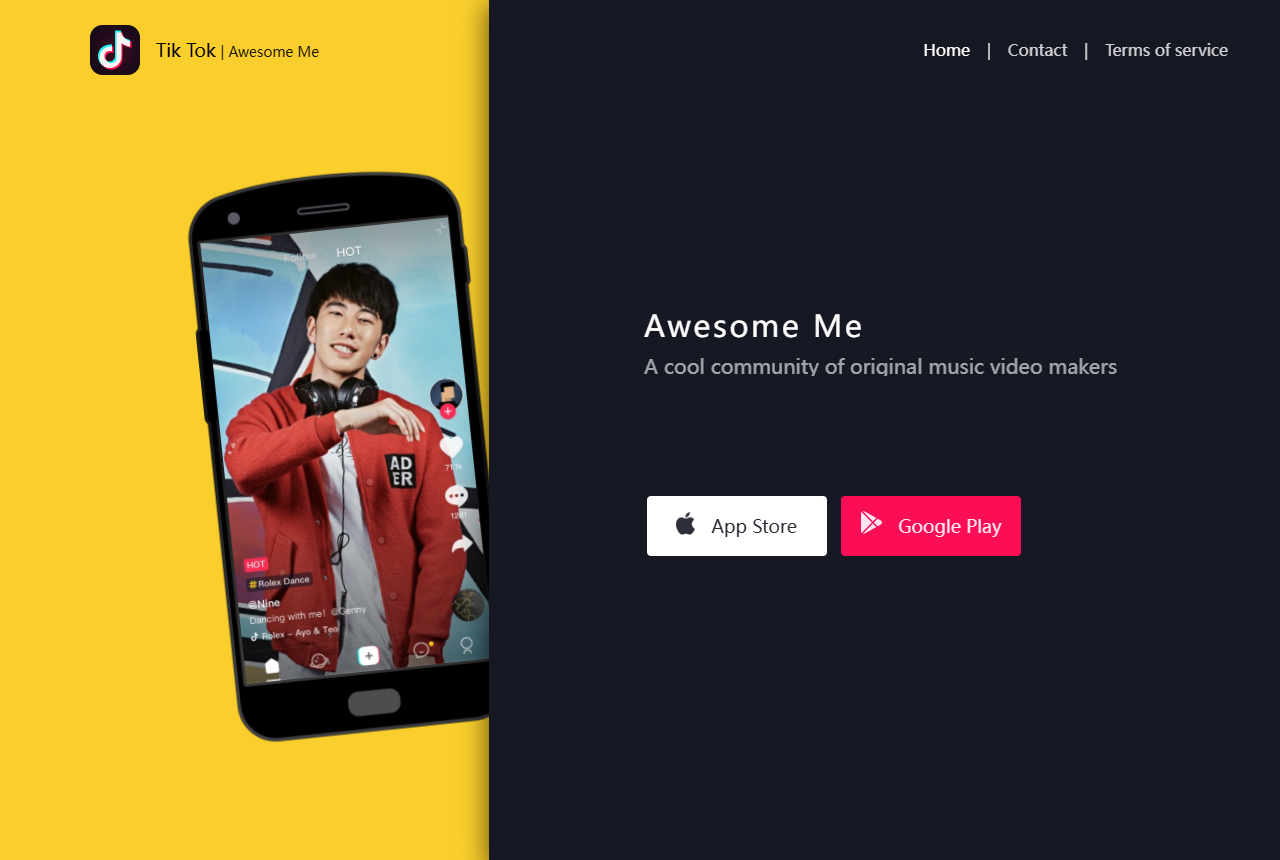
\includegraphics[height=4cm,keepaspectratio]{images/tiktok-2017.jpg}\\
{\tiny\color{gktmuted}Screenshot of TikTok in 2017. Web Design Museum, used with permission.}
\end{columns}
\end{frame}

% ============================================================
% 25 · CH12 ENVIRONMENTAL
% ============================================================
\begin{frame}{The Modern Gutta-Percha}
\begin{itemize}
\item CHOC titles this section \enquote{The Cloud as Utility and Platform} --- infrastructure at a scale the 2010s took for granted.
\item Same pattern as the transatlantic-cables story: convergence has a material substrate, usually invisible.
\item What was once millions of kilograms of gutta-percha is now data-center power and water.
\end{itemize}
\chaptertag{\enquote{The Cloud as Utility and Platform}}
\end{frame}

% ============================================================
% 26 · BRIDGE
% ============================================================
\begin{frame}{One More Entry in a Long List}
\begin{itemize}
\item From CHOC: the Turing machine, the memex, and the PC already extended human capability, long before anyone spoke of AI.
\item From my own course notes, a parallel list: the calculator, high-level languages and compilers, the Web, Wikipedia, and Stack Overflow each triggered the same \enquote{this makes programming knowledge unnecessary} anxiety --- and each time, \enquote{deep knowledge did not become obsolete; it became the thing that distinguished engineers who directed the tools well from those who were directed by them.} Generative AI is the latest entry, not a break from the pattern.
\item Same notes: \enquote{AI output is code, and code requires a reader.} Accountability stays human, as it did for all the others.
\end{itemize}
\noteinline{Two sources on this slide, kept deliberately distinct: CHOC's own augmentation throughline (bullet 1), and a course-reading argument of mine (bullets 2--3). CHOC ends in 2020, before generative AI.}
\chaptertag{Course notes cited: George K. Thiruvathukal, \enquote{A Pattern of Disruption? Or Yet Another Disruption?}, \emph{Introduction to Computer Science in Python: Principles and Practice} --- \url{introcs-python.cs.luc.edu/context/motivation.html}}
\end{frame}

% ============================================================
% 27 · PART 3 DIVIDER
% ============================================================
\section{Directing the Disruption}
\begin{frame}[plain]
\centering
{\Large\bfseries\color{gktaccent}Directing the Disruption}\\[1em]
\lead{\normalsize CHOC's territory ends in 2020. Computing has already disrupted culture, repeatedly, for twenty thousand years.}\\[1em]
{\normalsize Generative and agentic AI are the latest instance, not a category apart --- that claim is this talk's, not CHOC's.}
\end{frame}

% ============================================================
% 28 · RESOLVE FAUSTIAN-TURING
% ============================================================
\begin{frame}[plain]
\centering
{\Large\bfseries\color{gktaccent}The Hybrid We Already Are}\\[1em]
\begin{minipage}{0.8\textwidth}
\quoteblock{The resulting Faustian-Turing Type is both monstrous and marvelous, and we are it.}{\emph{History of Computing and Its Cultures}, resolving the figure introduced earlier in this talk}
\end{minipage}\\[1em]
\lead{\normalsize Not a doom narrative. A responsibility narrative.}\\[1em]
\chaptertag{\enquote{Conclusion: The Cultural-Computing Singularity}}
\end{frame}

% ============================================================
% 29 · 2020 HAND-OFF
% ============================================================
\begin{frame}{CHOC Ends Where This Talk Begins}
\begin{columns}[T]
\column{0.5\textwidth}
\centering
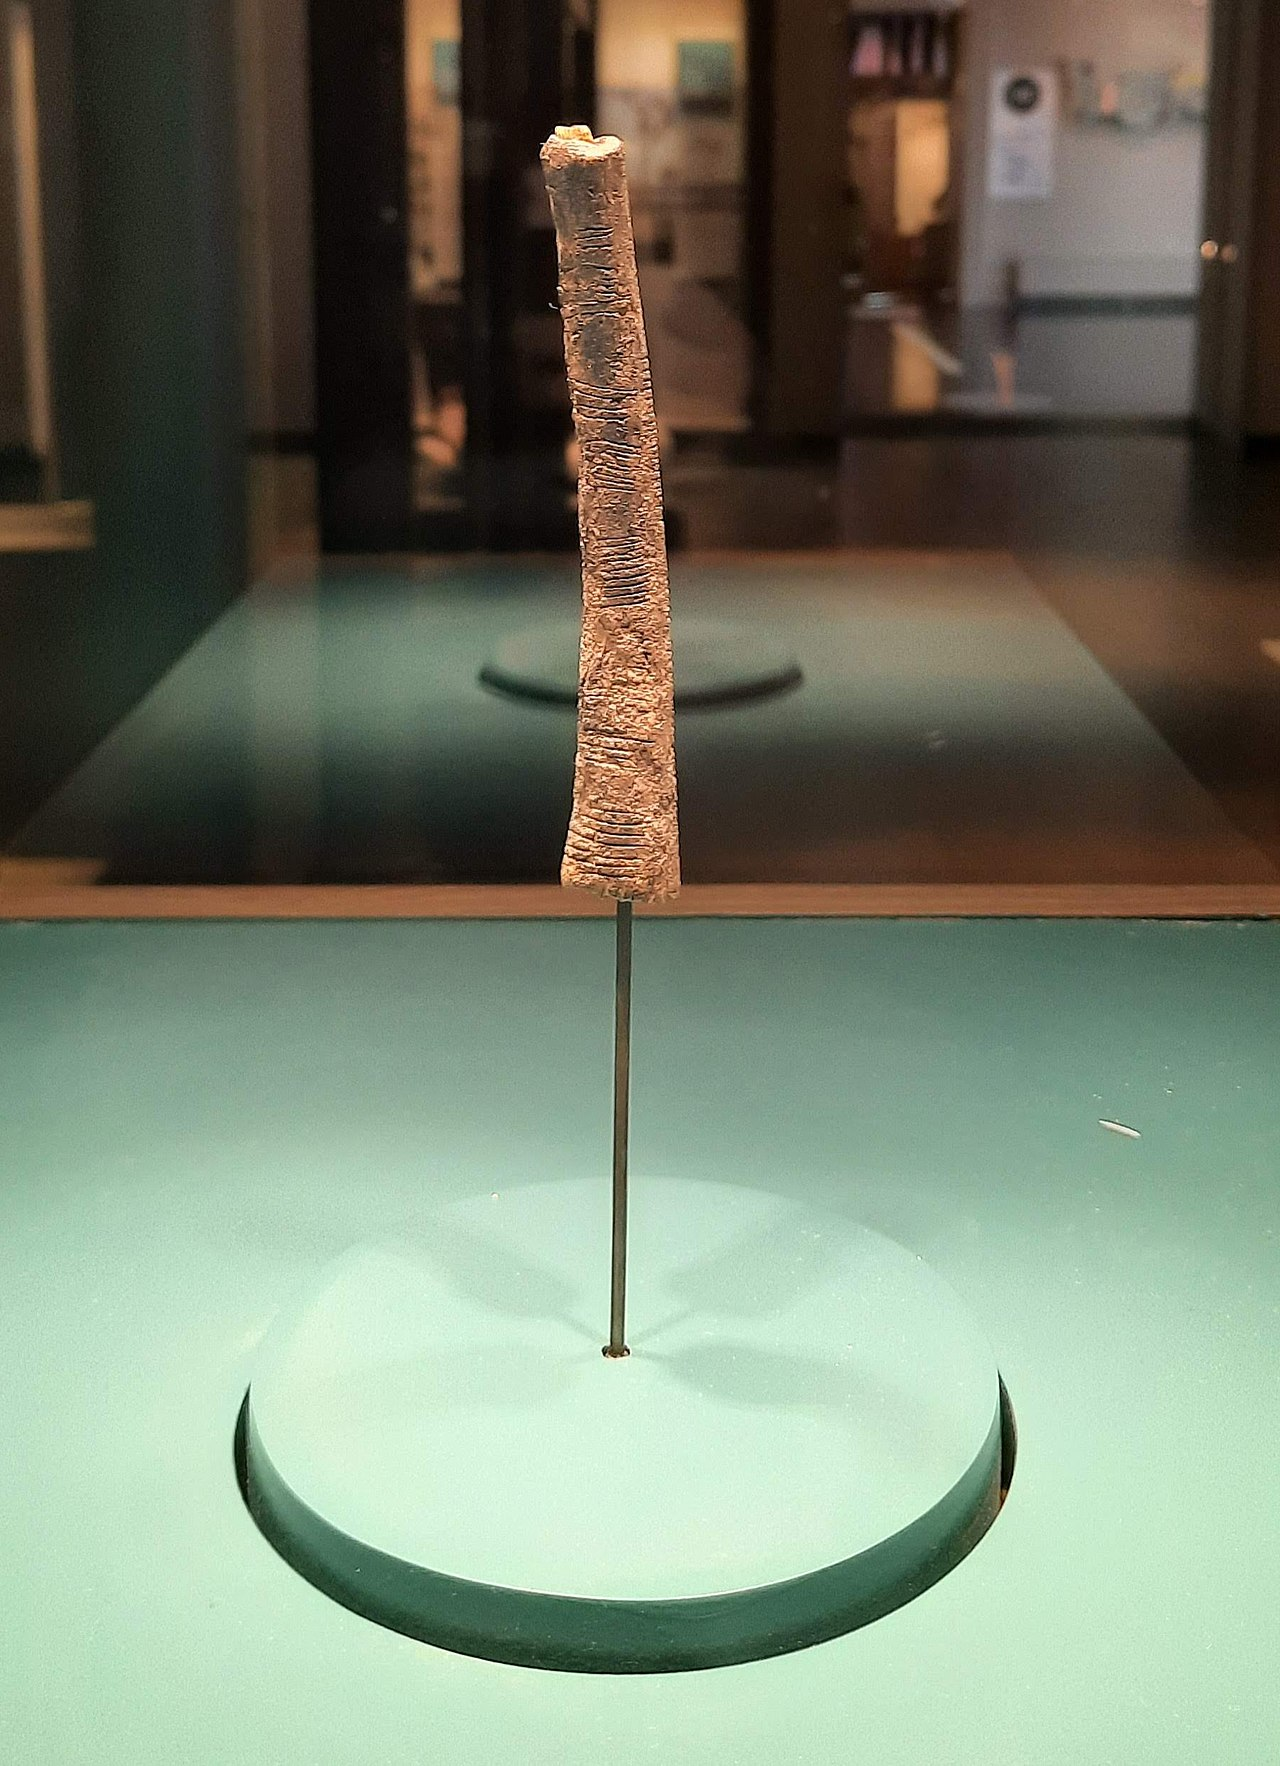
\includegraphics[height=3.2cm,keepaspectratio]{images/ishango-bone.jpg}\\
{\tiny\color{gktmuted}Ishango Bone. JhowieNitnek, Wikimedia Commons, CC BY-SA 4.0.}
\column{0.5\textwidth}
\centering
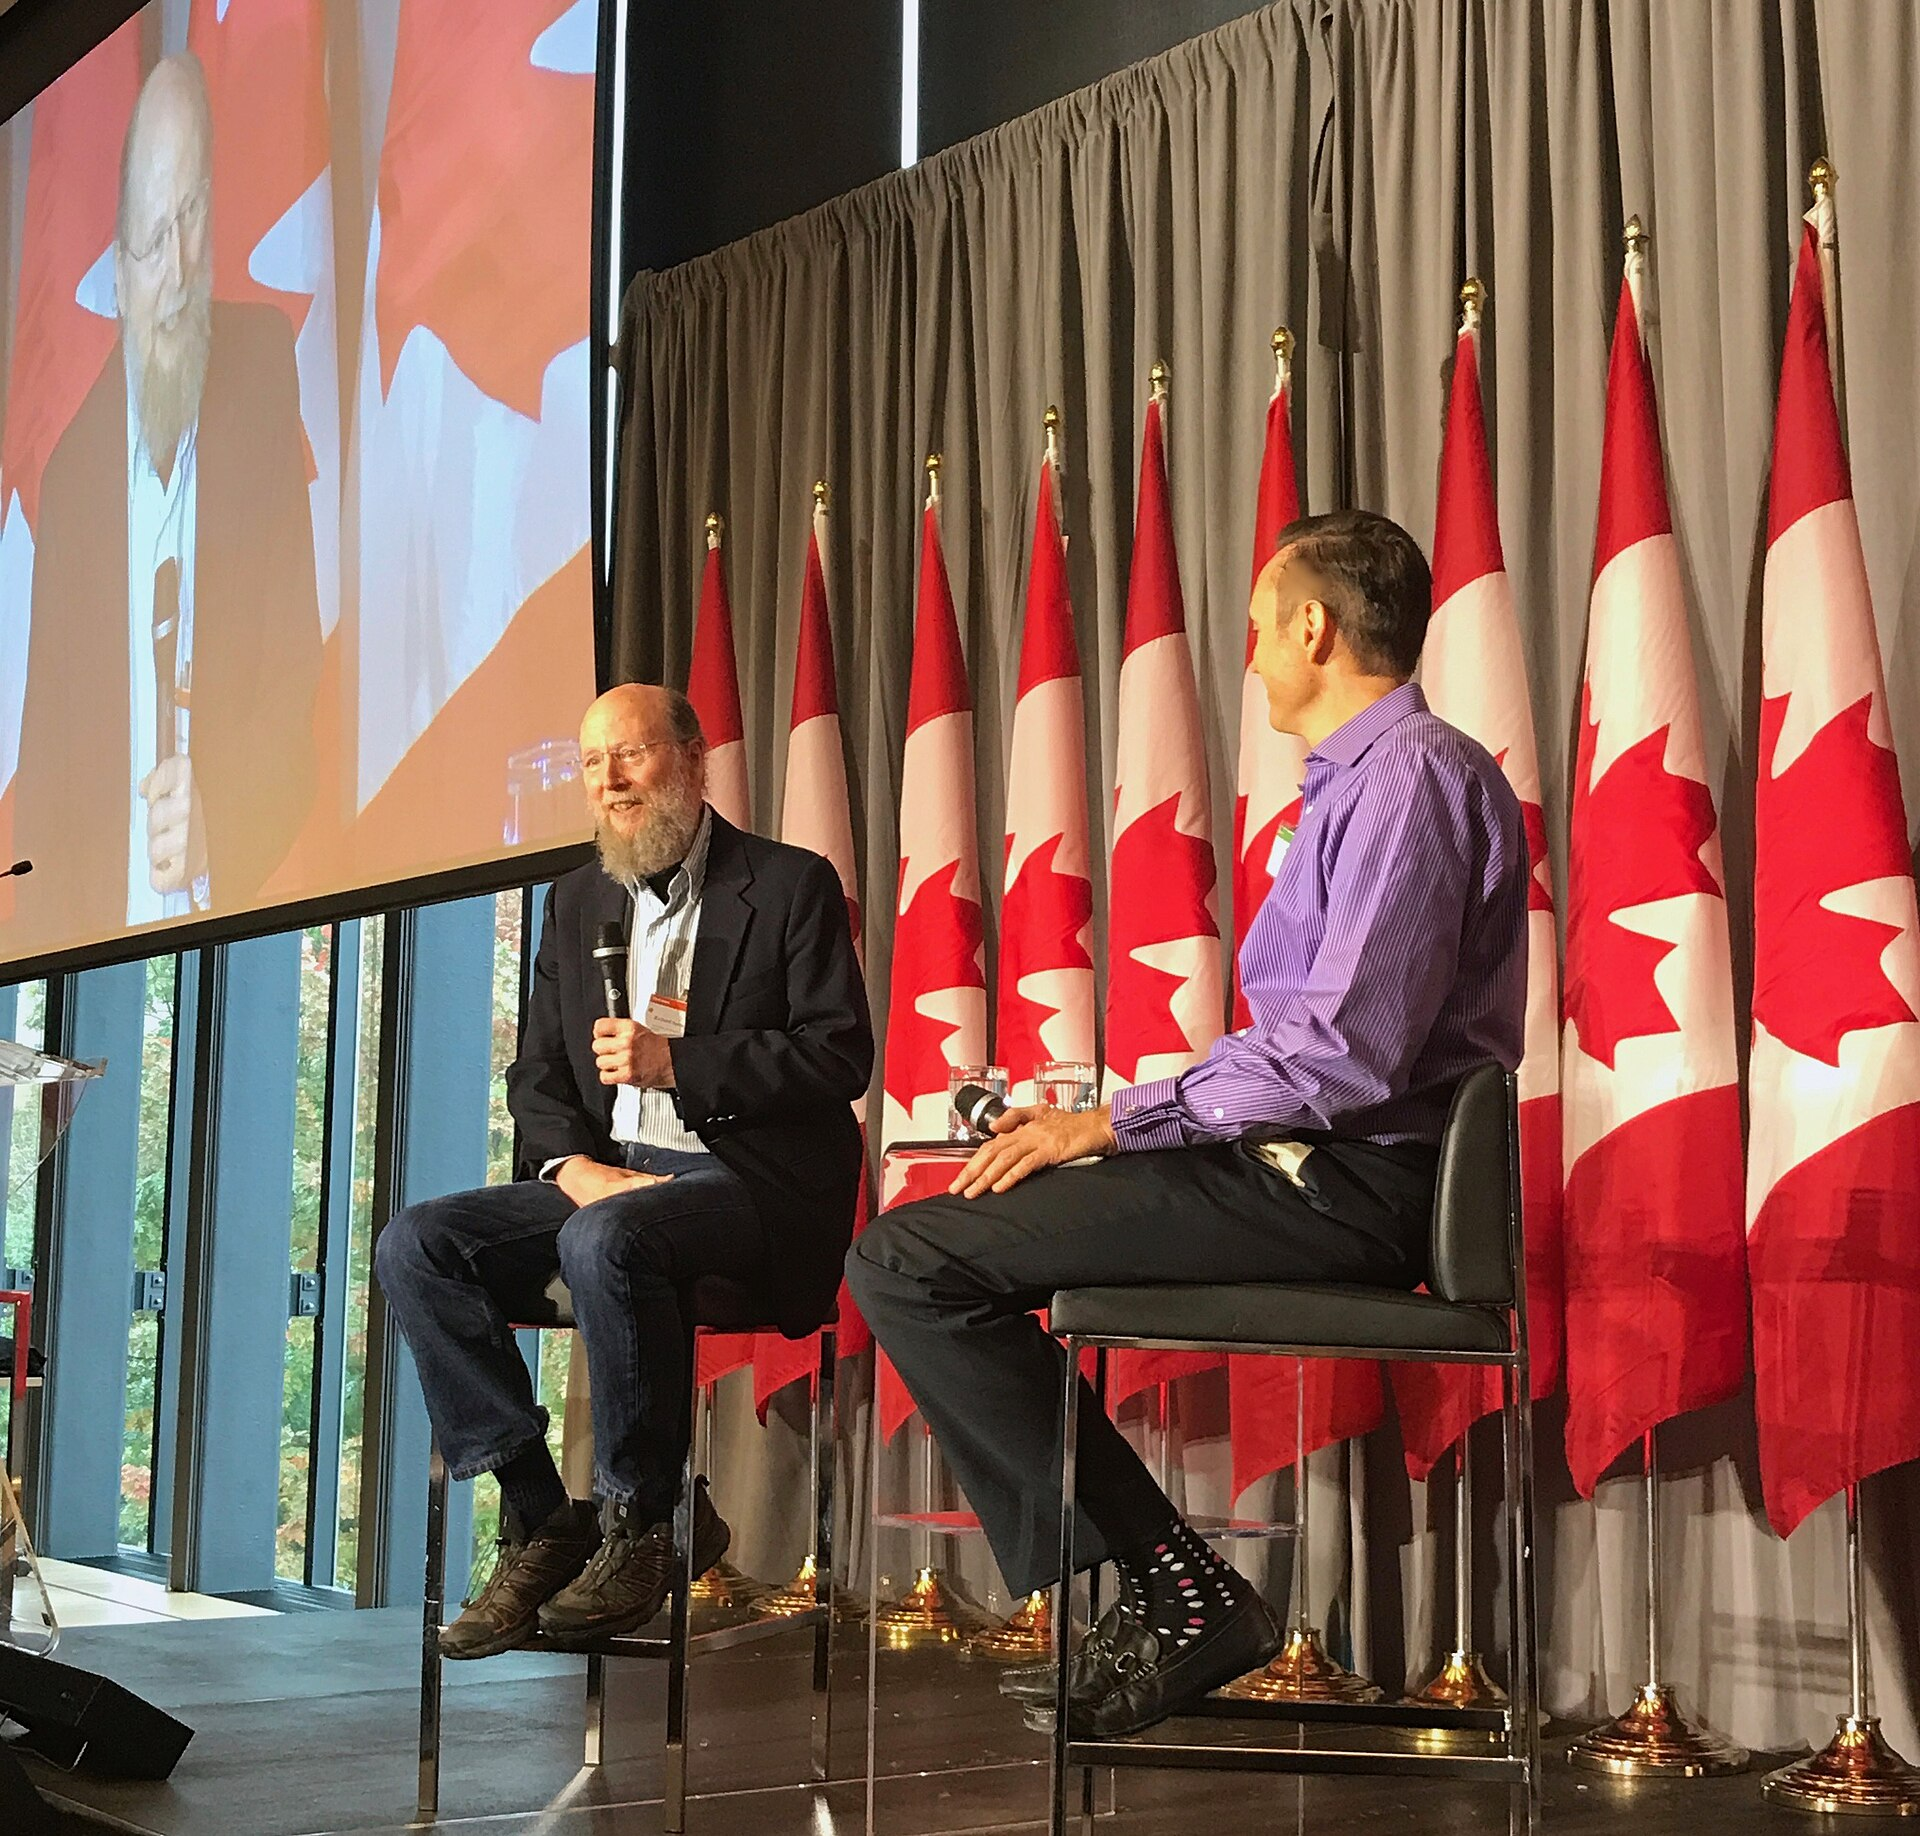
\includegraphics[height=3.2cm,keepaspectratio]{images/alpha-go.jpg}\\
{\tiny\color{gktmuted}AlphaGo / reinforcement learning. Wikimedia Commons, public domain.}
\end{columns}
\vspace{0.6em}
\begin{itemize}
\item CHOC's history runs from the Ishango Bone to 2020, and stops there deliberately.
\item Generative and agentic AI are the next, uncovered chapter --- not a rupture from what came before.
\end{itemize}
\chaptertag{\enquote{Conclusion: The Cultural-Computing Singularity}}
\end{frame}

% ============================================================
% 30 · PRACTICAL-HUMANIST CHARGE
% ============================================================
\begin{frame}{What CHOC Asks of Its Readers}
\quoteblock{The point is not that everyone must become a computer scientist\ldots{} To ride the currents of change rather than be swamped by them requires a working understanding of how these systems shape production, distribution, discovery, and memory.}{\emph{History of Computing and Its Cultures}, closing charge to readers}
\chaptertag{\enquote{Conclusion: The Cultural-Computing Singularity}}
\end{frame}

% ============================================================
% 31 · CLOSING
% ============================================================
\begin{frame}[plain]
\centering
{\Large\bfseries\color{gktaccent}Computing Has Always Disrupted Culture}\\[1em]
\lead{\normalsize That's CHOC's evidence --- twenty thousand years, no exception.}\\[1em]
\begin{minipage}{0.85\textwidth}
\normalsize Generative and agentic AI are not a rupture from that pattern; they are its newest instance. The question is whether we can direct the disruption toward human flourishing --- while retaining the knowledge, judgment, and responsibility to remain meaningful agents in an increasingly computational culture.
\end{minipage}\\[1.4em]
{\normalsize George K. Thiruvathukal \quad$\cdot$\quad David B. Dennis}
\end{frame}

% ============================================================
% 32 · QR CODES (closing, identical to post-title frame)
% ============================================================
\begin{frame}[plain]
\centering
{\Large\bfseries\color{gktaccent}Follow Along}\\[1em]
\begin{columns}[T]
\column{0.5\textwidth}
\centering

\includegraphics[height=3.6cm]{images/qr-talk.png}\\[0.4em]
\footnotesize This talk\\\href{https://talks.gkt.sh/luc-digital-ethics-2026/}{talks.gkt.sh/luc-digital-ethics-2026}
\column{0.5\textwidth}
\centering

\includegraphics[height=3.6cm]{images/qr-keylinks.png}\\[0.4em]
\footnotesize Find me\\\href{https://keylinks.gkt.sh}{keylinks.gkt.sh}
\end{columns}
\end{frame}

\end{document}
